\documentclass[]{book}
\usepackage{lmodern}
\usepackage{amssymb,amsmath}
\usepackage{ifxetex,ifluatex}
\usepackage{fixltx2e} % provides \textsubscript
\ifnum 0\ifxetex 1\fi\ifluatex 1\fi=0 % if pdftex
  \usepackage[T1]{fontenc}
  \usepackage[utf8]{inputenc}
\else % if luatex or xelatex
  \ifxetex
    \usepackage{mathspec}
  \else
    \usepackage{fontspec}
  \fi
  \defaultfontfeatures{Ligatures=TeX,Scale=MatchLowercase}
\fi
% use upquote if available, for straight quotes in verbatim environments
\IfFileExists{upquote.sty}{\usepackage{upquote}}{}
% use microtype if available
\IfFileExists{microtype.sty}{%
\usepackage{microtype}
\UseMicrotypeSet[protrusion]{basicmath} % disable protrusion for tt fonts
}{}
\usepackage[margin=1in]{geometry}
\usepackage{hyperref}
\PassOptionsToPackage{usenames,dvipsnames}{color} % color is loaded by hyperref
\hypersetup{unicode=true,
            pdftitle={Simulación y analisis de ocupación},
            pdfauthor={Diego J. Lizcano},
            colorlinks=true,
            linkcolor=blue,
            citecolor=Blue,
            urlcolor=Blue,
            breaklinks=true}
\urlstyle{same}  % don't use monospace font for urls
\usepackage{natbib}
\bibliographystyle{plainnat}
\usepackage{color}
\usepackage{fancyvrb}
\newcommand{\VerbBar}{|}
\newcommand{\VERB}{\Verb[commandchars=\\\{\}]}
\DefineVerbatimEnvironment{Highlighting}{Verbatim}{commandchars=\\\{\}}
% Add ',fontsize=\small' for more characters per line
\usepackage{framed}
\definecolor{shadecolor}{RGB}{248,248,248}
\newenvironment{Shaded}{\begin{snugshade}}{\end{snugshade}}
\newcommand{\KeywordTok}[1]{\textcolor[rgb]{0.13,0.29,0.53}{\textbf{{#1}}}}
\newcommand{\DataTypeTok}[1]{\textcolor[rgb]{0.13,0.29,0.53}{{#1}}}
\newcommand{\DecValTok}[1]{\textcolor[rgb]{0.00,0.00,0.81}{{#1}}}
\newcommand{\BaseNTok}[1]{\textcolor[rgb]{0.00,0.00,0.81}{{#1}}}
\newcommand{\FloatTok}[1]{\textcolor[rgb]{0.00,0.00,0.81}{{#1}}}
\newcommand{\ConstantTok}[1]{\textcolor[rgb]{0.00,0.00,0.00}{{#1}}}
\newcommand{\CharTok}[1]{\textcolor[rgb]{0.31,0.60,0.02}{{#1}}}
\newcommand{\SpecialCharTok}[1]{\textcolor[rgb]{0.00,0.00,0.00}{{#1}}}
\newcommand{\StringTok}[1]{\textcolor[rgb]{0.31,0.60,0.02}{{#1}}}
\newcommand{\VerbatimStringTok}[1]{\textcolor[rgb]{0.31,0.60,0.02}{{#1}}}
\newcommand{\SpecialStringTok}[1]{\textcolor[rgb]{0.31,0.60,0.02}{{#1}}}
\newcommand{\ImportTok}[1]{{#1}}
\newcommand{\CommentTok}[1]{\textcolor[rgb]{0.56,0.35,0.01}{\textit{{#1}}}}
\newcommand{\DocumentationTok}[1]{\textcolor[rgb]{0.56,0.35,0.01}{\textbf{\textit{{#1}}}}}
\newcommand{\AnnotationTok}[1]{\textcolor[rgb]{0.56,0.35,0.01}{\textbf{\textit{{#1}}}}}
\newcommand{\CommentVarTok}[1]{\textcolor[rgb]{0.56,0.35,0.01}{\textbf{\textit{{#1}}}}}
\newcommand{\OtherTok}[1]{\textcolor[rgb]{0.56,0.35,0.01}{{#1}}}
\newcommand{\FunctionTok}[1]{\textcolor[rgb]{0.00,0.00,0.00}{{#1}}}
\newcommand{\VariableTok}[1]{\textcolor[rgb]{0.00,0.00,0.00}{{#1}}}
\newcommand{\ControlFlowTok}[1]{\textcolor[rgb]{0.13,0.29,0.53}{\textbf{{#1}}}}
\newcommand{\OperatorTok}[1]{\textcolor[rgb]{0.81,0.36,0.00}{\textbf{{#1}}}}
\newcommand{\BuiltInTok}[1]{{#1}}
\newcommand{\ExtensionTok}[1]{{#1}}
\newcommand{\PreprocessorTok}[1]{\textcolor[rgb]{0.56,0.35,0.01}{\textit{{#1}}}}
\newcommand{\AttributeTok}[1]{\textcolor[rgb]{0.77,0.63,0.00}{{#1}}}
\newcommand{\RegionMarkerTok}[1]{{#1}}
\newcommand{\InformationTok}[1]{\textcolor[rgb]{0.56,0.35,0.01}{\textbf{\textit{{#1}}}}}
\newcommand{\WarningTok}[1]{\textcolor[rgb]{0.56,0.35,0.01}{\textbf{\textit{{#1}}}}}
\newcommand{\AlertTok}[1]{\textcolor[rgb]{0.94,0.16,0.16}{{#1}}}
\newcommand{\ErrorTok}[1]{\textcolor[rgb]{0.64,0.00,0.00}{\textbf{{#1}}}}
\newcommand{\NormalTok}[1]{{#1}}
\usepackage{longtable,booktabs}
\usepackage{graphicx,grffile}
\makeatletter
\def\maxwidth{\ifdim\Gin@nat@width>\linewidth\linewidth\else\Gin@nat@width\fi}
\def\maxheight{\ifdim\Gin@nat@height>\textheight\textheight\else\Gin@nat@height\fi}
\makeatother
% Scale images if necessary, so that they will not overflow the page
% margins by default, and it is still possible to overwrite the defaults
% using explicit options in \includegraphics[width, height, ...]{}
\setkeys{Gin}{width=\maxwidth,height=\maxheight,keepaspectratio}
\IfFileExists{parskip.sty}{%
\usepackage{parskip}
}{% else
\setlength{\parindent}{0pt}
\setlength{\parskip}{6pt plus 2pt minus 1pt}
}
\setlength{\emergencystretch}{3em}  % prevent overfull lines
\providecommand{\tightlist}{%
  \setlength{\itemsep}{0pt}\setlength{\parskip}{0pt}}
\setcounter{secnumdepth}{5}
% Redefines (sub)paragraphs to behave more like sections
\ifx\paragraph\undefined\else
\let\oldparagraph\paragraph
\renewcommand{\paragraph}[1]{\oldparagraph{#1}\mbox{}}
\fi
\ifx\subparagraph\undefined\else
\let\oldsubparagraph\subparagraph
\renewcommand{\subparagraph}[1]{\oldsubparagraph{#1}\mbox{}}
\fi

%%% Use protect on footnotes to avoid problems with footnotes in titles
\let\rmarkdownfootnote\footnote%
\def\footnote{\protect\rmarkdownfootnote}

%%% Change title format to be more compact
\usepackage{titling}

% Create subtitle command for use in maketitle
\newcommand{\subtitle}[1]{
  \posttitle{
    \begin{center}\large#1\end{center}
    }
}

\setlength{\droptitle}{-2em}
  \title{Simulación y analisis de ocupación}
  \pretitle{\vspace{\droptitle}\centering\huge}
  \posttitle{\par}
\subtitle{Entendiendo las simulaciones y el modelo básico. Gran parte del código y
el texto han sido adaptados de los libros de Marc Kery (2010, 2011, y
2015)}
  \author{Diego J. Lizcano}
  \preauthor{\centering\large\emph}
  \postauthor{\par}
  \predate{\centering\large\emph}
  \postdate{\par}
  \date{2016-08-31}

\usepackage{booktabs}

\begin{document}
\maketitle

{
\hypersetup{linkcolor=black}
\setcounter{tocdepth}{1}
\tableofcontents
}
\chapter{Prerequisitos}\label{prerequisitos}

This is a \emph{sample} book written in \textbf{Markdown} con los
paquetes `bookdown', `knitr'y 'rmarkdown'.

Antes de comenzar por favor instale el programa JAGS en su computadora,
posteriormente desde R studio instale los paquetes unmarked, raster,
statspat y jagsUI

\begin{Shaded}
\begin{Highlighting}[]
\KeywordTok{install.packages}\NormalTok{(}\StringTok{"unmarked"}\NormalTok{, }\DataTypeTok{dependencies =} \OtherTok{TRUE}\NormalTok{)}
\KeywordTok{install.packages}\NormalTok{(}\StringTok{"raster"}\NormalTok{, }\StringTok{"statspat"}\NormalTok{, }\StringTok{"jagsUI"}\NormalTok{, }\DataTypeTok{dependencies =} \OtherTok{TRUE}\NormalTok{)}
\end{Highlighting}
\end{Shaded}

\chapter{Introducion}\label{intro}

Simulación de datos de ocupación, bajo el modelo estático (MacKenzie et
al. 2002) para el venado de cola blanca en el Parque Nacional
Machalilla.

El objetivo de este documento es entender la versatilidad y el poder de
las simulaciones con R en el capitulo @ref(why\_sumul), para aprender
como funciona y el modelo básico de ocupacion \ref{occu} con un ejemplo
sencillo \ref{example} del PN Machalilla. Posteriormente empacaremos el
codigo que genera datos de ocupacion en una sola funcion \ref{funcion1},
la cual nos permitira simular datos bajo diferentes escenarios, que
analizaremos con la funcion occu del paquete unmarked \ref{unmarked}.
Posteriormente analizaremos los mismos datos bajo estimadores bayesianos
\ref{bayesian}

Gran parte del concepto, el código y el texto han sido adaptados de los
libros de Marc Kery \citep{Kery2012}, \citep{Kery2011a},
\citep{Kery2010}, \citep{kery2015applied}.

\chapter{Porque simular?}\label{why_sumul}

\section{Por que son útiles las
simulaciones:}\label{por-que-son-utiles-las-simulaciones}

\begin{enumerate}
\def\labelenumi{\arabic{enumi}.}
\tightlist
\item
  Al hacer simulaciones se conocen los parámetros verdaderos, así que
  podremos asegurarnos que el código que ejecutamos (R o BUGS) estima lo
  que queremos, y que los estimados son iguales o se acercan a los
  parámetros verdaderos, permitiendo depurar errores en el código.
\item
  Podemos calibrar un modelo derivado y/o más complejo más fácilmente.
  Las simulaciones pueden ser vistas como un experimento controlado, o
  como versiones simplificadas de un sistema real, en el cual podemos
  probar como varían ciertos parámetros que afectan los estimados de
  otros parámetros. Realizar experimentos controlados en el mundo real
  es muchas veces impractico o imposible en ecología, así que la
  simulación es la forma mas coherente de estudiar el sistema ecológico.
\item
  Se experimenta de primera mano el error de muestreo y se convierte en
  un fantástico proceso de aprendizaje.
\item
  Podemos verificar la calidad (frecuentista) de los estimados, así como
  la precisión y el efecto del tamaño muestral, computando la diferencia
  entre la media del estimado y el valor real (sesgo) y la varianza del
  estimado (la precisión).
\item
  Es la forma más flexible y directa de realizar un análisis de poder,
  resolviendo el gran problema de determinar el tamaño de la muestra
  necesario para detectar un efecto de cierta magnitud, con una
  probabilidad dada.\\
\item
  Podemos visualizar que tan identificables son los parámetros en
  modelos más complejos.
\item
  Podemos verificar que tan robusto es el modelo a violaciones de lo que
  se asume.
\item
  Al ser capaces de simular datos bajo cierto modelo, se garantiza que
  uno entiende el modelo, sus restricciones y limitaciones.
\end{enumerate}

\chapter{La ocupación de hábitat}\label{occu}

Obtener datos para estudios de poblaciones animales, es costoso y
dispendioso, y no siempre se puede medir la densidad poblacional o
parámetros demográficos como natalidad o mortalidad. Es por eso que la
estimación de ocupación de hábitat (\(\psi\)) es una buena herramienta
de estudio, ya que es un reflejo de otros parámetros poblacionales
importantes como la abundancia y densidad, que requieren de un elevado
número de registros, con los costos económicos y logísticos que
conlleva. Adicionalmente y debido a que la detectabilidad (\emph{p}) en
animales silvestres no es completa, el uso de los datos crudos genera
subestimaciones de la ocupación de hábitat. Con el empleo de muestreos
repetidos, es posible generar estimaciones de detectabilidad y, con esta
estimación, obtener valores no sesgados de la ocupación del hábitat. Los
métodos de análisis de la ocupación fueron inicialmente desarollados por
\citet{MacKenzie2002} y posteriormente expandidos por otros autores
\citep{MACKENZIE2005, MacKenzie2006, Kery2008, Royle2007a, Royle2005, Royle2006}.
Este tipo de modelos permiten realizar inferencias acerca de los efectos
de variables continuas y categóricas sobre la ocupación de hábitat.
Además, si los muestreos se realizan a través de períodos largos de
tiempo, también es posible estimar tasas de extinción y recolonización,
que son útiles en estudios de metapoblaciones \citep{MacKenzie2003}.
Este es un campo de gran desarrollo en bioestadística que ha producido
una gran explosión de estudios que usan la ocupación teniendo en cuenta
la detectabilidad
\citep{Guillera-Arroita2010a, Guillera-Arroita2015, Guillera-Arroita2011, Guillera-Arroita2012, Guillera-Arroita2014a, Kery2013}.

\chapter{Nuestro ejemplo:}\label{example}

El set de datos que vamos a simular, imita la forma espacial y temporal
como imaginamos se originan las medidas repetidas de presencia ausencia
en ecología. Las cuales son una combinación de un proceso ecológico y un
proceso de observación. El primer proceso contiene los mecanismos bajos
los cuales se originan patrones espacio-temporales de distribución,
mientras que el segundo proceso contiene las diferentes facetas en las
cuales se originan fuentes de error al tomar los datos.

Para ser más concretos vamos a llamar a nuestra especie imaginaria con
un nombre real. La llamaremos el venado de cola blanca (\emph{Odocoileus
virginianus}), un mamífero grande y común, ampliamente distribuido en el
continente Americano, y de preocupación menor en términos de
\href{http://www.iucnredlist.org/details/42394}{conservación}.

\includegraphics{http://static.inaturalist.org/photos/1305358/large.JPG?1414422110}
El Venado de cola blanca (\emph{Odocoileus virginianus}) nuestra especie
de interes para este ejemplo. Foto del proyecto fauna de Manabi
\url{http://faunamanabi.github.io}

El set de datos contiene \emph{J} datos replicados de detección o no
detección de la especie en \emph{M} sitios, teniendo en cuenta que
asumimos que es una población cerrada (`closure' assumption). Es decir
que durante el muestreo no ocurrieron cambios por nacimientos, muertes
inmigración o emigración. En otras palabras, el muestreo fue corto en
tiempo y la ocurrencia de la especie \emph{z} no cambió por efectos
demográficos.

Claramente debemos distinguir dos procesos, el primero es el proceso
ecológico, el cual genera (parcialmente) un estado latente de la
ocurrencia \emph{z}. El segundo es el proceso de observación, el cual
produce los datos observados de detección o no detección del venado.
Aquí asumimos que el proceso de observación está gobernado por un
mecanismo de detección imperfecta. Es decir algunos venado pudieron
haberse escapado a mi observación, lo cual genera falsos negativos.
También asumimos que los falsos positivos están ausentes, es decir que
todo lo que identifico como venado, es efectivamente un venado. Para
hacer más realista el ejemplo incluimos los efectos de la altitud y la
cobertura de bosque en la ocurrencia, como factores que afectan la
ocurrencia linealmente, disminuyendola para el caso de la elevación y
que incrementan la ocupación linealmente para el caso de la cobertura de
bosques. Al final las dos variables interactúan negativamente entre sí.
Esos efectos se introducen en la ocurrencia en escala logarítmica como
tradicionalmente se hace un modelo lineal generalizado (GLM).

En nuestra simulación vamos a hacer explícito que no es posible detectar
a la totalidad de los venados de un sitio de muestreo, así que estamos
enfrentando un tipo de error que nos hace sub-estimar la abundancia de
la población. Hay muchas razónes por las cuales fallamos en detectar un
individuo en la naturaleza, porque nos distrajimos mientras el venado
paso, porque los binoculares no tenían el aumento suficiente, o
simplemente porque el venado se escondió detrás de un árbol al sentir
nuestro olor, o por alguna otra razón. De esta forma nosotros vamos a
registrar la presencia (\emph{z}=1) con una probabilidad de detección
\emph{p} la cual también vamos a hacerla dependiente (en la escala
logarítmica) de la altitud y de una co-variable que afecta la detección,
la temperatura. En términos generales los animales son más difíciles de
observar cuando la temperatura es mas alta y por lo general entre más
altitud la temperatura disminuye. De esta forma asumimos que la
detección está relacionada negativamente con a con la altitud y la
temperatura. Pero también hay que tener en cuenta que el efecto negativo
en \emph{p} también puede ser mediado por una disminución en la
abundancia con la altitud, el cual también causa que la probabilidad de
ocupación disminuya con la altitud. Tenga en cuenta que una co-variable,
la altitud afecta a ambos procesos, el ecológico (la ocurrencia) y al
proceso de observación (la probabilidad de detección). Esto tiene un
propósito, y es probable que pase en la naturaleza muchas veces. Los
modelos de ocupación tienen una base ``mecanistica'' produciendo
variación espacial en la abundancia. Es decir tendremos sitios con mayor
abundancia y otros con menor abundancia. Pero los modelos jerárquicos
como el que estamos por construir, son capaces de desentrañar esas
relaciones complejas entre ocurrencia y probabilidad de detección
\citep{Kery2008, KERY2008, Kery2012}. Finalmente para este primer
ejemplo vamos a dejar por fuera el efecto de la interacción entre la
altitud y la temperatura, ajustándolo a cero. Luego podremos variar este
parámetro para considerar ese efecto. En resumen vamos a generar datos
bajo el siguiente modelo, donde los sitios son indexados como \emph{i} y
los conteos repetidos en el sitio van a ser referidos como \emph{j}.

\subsection{Modelo Ecológico:}\label{modelo-ecologico}

\(z _{i} = Bernoulli (\psi _{i})\)

\(logit(\psi _{i}) = \beta _{0} + \beta _{1} \ast Altitud _{i} + \beta _{2}\ast CovBosque _{i} + \beta _{3} \ast Altitud _{i} \ast CovBosque _{i}\)

\subsection{Modelo de Observación:}\label{modelo-de-observacion}

\(y _{ij} = Bernoulli (z _{i} * p _{ij})\)

\(logit(p _{ij}) = \alpha _{0} + \alpha _{1} \ast Altitud _{i} + \alpha _{2}\ast Temperatura _{ij} + \alpha _{3} \ast Altitud _{i} \ast Temperatura _{ij}\)

Donde \(\psi\) es la ocupación y \emph{p} la probabilidad de detección.
Con \(\beta\) como el coeficiente de la regresión para las co-variables
de la ocupación y \(\alpha\) el coeficiente de regresión para las
co-variables de la detección.

Vamos a generar datos desde ``dentro hacia afuera'' y desde arriba hacia
abajo. Para esto, primero escogemos el tamaño de la muestra y creamos
los valores para las co-variables. Segundo, seleccionamos los valores de
los parámetros de del modelo ecológico (la ocupación) y ensamblamos la
ocurrencia esperada (el parámetro \(\psi\), o la ocupación) y
posteriormente obtenemos la variable al azar \emph{z} la cual tiene
distribución Bernoulli. Tercero, seleccionamos los valores de los
parámetros del modelo de observación (la detección), para ensamblar la
probabilidad de detección \emph{p} y obtener el segundo set de una
variable al azar \emph{y} (detección observada o no observada de un
venado) la cual también tiene distribución Bernoulli.

Para simular los datos usaremos el lenguaje de programación estadística
R \citep{RCoreTeam2016}, el cual provee una gran variedad de técnicas
gráficas y estadísticas de modelación y un gran ecosistema de paquetes
para análisis estadístico y ecológico. Si aún no lo ha hecho, baje e
instale \href{http://www.r-project.org/}{R} en su computadora,
posteriormente haga lo mismo con
\href{http://www.rstudio.com/}{RStudio.}

\section{Pasos iniciales: tamaño de la muestra y valores de las
co-variables}\label{pasos-iniciales-tamano-de-la-muestra-y-valores-de-las-co-variables}

Inicie \href{http://www.rstudio.com/}{RStudio}, copie, pegue y ejecute
los comandos de la ventana gris.

Primero escogemos el tamaño de la muestra, el número de sitios y el
número de medidas repetidas (número de visitas) de presencia/ausencia en
cada sitio.

\begin{Shaded}
\begin{Highlighting}[]
\NormalTok{M <-}\StringTok{ }\DecValTok{60}  \CommentTok{# Número de réplicas espaciales (sitios)}
\NormalTok{J <-}\StringTok{ }\DecValTok{30}  \CommentTok{# Número de réplicas temporales (conteos repetidos)}
\end{Highlighting}
\end{Shaded}

Luego creamos los valores para las co-variables. Tenemos altitud y
cobertura de bosque como co-variables de cada sitio. Ellas difieren de
sitio a sitio pero para cada muestreo son las mismas. Mientras que la
temperatura es una co-variable de la observación, así que si varía en
cada muestreo y también en cada sitio. Recuerde que el sub índice
\emph{i} se refiere al sitio y el \emph{j} a cada muestreo. Para
simplificar las cosas nuestras co-variables van a tener una distribución
normal con una media centrada en cero y no se van a extender muy lejos
en cada lado del cero. En análisis de datos reales tendremos que
estandarizar las co-variables para evitar problemas numéricos de
diferencia en las escalas de las co-variables y poder calcular el valor
de máxima verosimilitud (ML), así como también para obtener convergencia
en las cadenas de Markov del modelo Bayesiano. Aquí vamos a ignorar un
hecho de la vida real, y es que las co-variables no son totalmente
independientes la una de la otra, es decir en la naturaleza la cobertura
boscosa puede estar relacionada con la altitud, pero esto no va a ser
relevante, por ahora.

Para inicializar el generador de números aleatorios y obtener siempre
los mismos resultados podemos adicionar la siguiente línea:

\begin{Shaded}
\begin{Highlighting}[]
\KeywordTok{set.seed}\NormalTok{(}\DecValTok{24}\NormalTok{) }\CommentTok{# Can choose seed of your choice}
\end{Highlighting}
\end{Shaded}

De esta forma podremos obtener siempre los mismos estimados. Pero luego
cuando queramos obtener el error de muestreo deberemos remover esa
línea. Para este ejemplo generaremos valores para las covariables
centrados en cero y variando de -1 a 1.

\begin{Shaded}
\begin{Highlighting}[]
\NormalTok{elev <-}\StringTok{ }\KeywordTok{runif}\NormalTok{(}\DataTypeTok{n =} \NormalTok{M, -}\DecValTok{1}\NormalTok{, }\DecValTok{1}\NormalTok{)             }\CommentTok{# Scaled elevation of a site}
\NormalTok{forest <-}\StringTok{ }\KeywordTok{runif}\NormalTok{(}\DataTypeTok{n =} \NormalTok{M, -}\DecValTok{1}\NormalTok{, }\DecValTok{1}\NormalTok{)           }\CommentTok{# Scaled forest cover at each site}
\NormalTok{temp <-}\StringTok{ }\KeywordTok{array}\NormalTok{(}\KeywordTok{runif}\NormalTok{(}\DataTypeTok{n =} \NormalTok{M*J, -}\DecValTok{1}\NormalTok{, }\DecValTok{1}\NormalTok{), }\DataTypeTok{dim =} \KeywordTok{c}\NormalTok{(M, J)) }\CommentTok{# Scaled temperature}
\end{Highlighting}
\end{Shaded}

\section{Simulando el proceso ecológico y su resultado: la ocurrencia
del
venado}\label{simulando-el-proceso-ecologico-y-su-resultado-la-ocurrencia-del-venado}

Para simular la ocurrencia del venado en cada sitio, escogemos los
valores para los parámetros que gobiernan la variación espacial en la
ocurrencia \(\beta _{0}\) a \(\beta _{3}\). El primer parámetro es la
ocurrencia promedio esperada del venado (probabilidad de ocupación)
cuando todas las co-variables tienen un valor de cero, en otras palabras
el intercepto del modelo de ocurrencia. Preferimos pensar en los venados
en términos de su ocurrencia en lugar de logit(ocurrencia). Aquí
nosotros escogemos el intercepto de la ocupación primero y luego lo
transformamos de la escala logarítmica con la función de enlace logit.

\begin{Shaded}
\begin{Highlighting}[]
\NormalTok{mean.occupancy <-}\StringTok{ }\FloatTok{0.60}         \CommentTok{# Mean expected occurrence of deer}
\NormalTok{beta0 <-}\StringTok{ }\KeywordTok{plogis}\NormalTok{(mean.occupancy) }\CommentTok{# Same on logit scale (= logit-scale intercept)}
\NormalTok{beta1 <-}\StringTok{ }\NormalTok{-}\DecValTok{2}                    \CommentTok{# Effect (slope) of elevation}
\NormalTok{beta2 <-}\StringTok{ }\DecValTok{2}                     \CommentTok{# Effect (slope) of forest cover}
\NormalTok{beta3 <-}\StringTok{ }\DecValTok{1}                     \CommentTok{# Interaction effect (slope) of elev and forest}
\end{Highlighting}
\end{Shaded}

Aquí aplicamos el modelo lineal (a la escala logarítmica) y obtenemos la
transformación logit de la probabilidad de ocupación, la cual invertimos
con la transformación logit para obtener la ocupación del venado y
graficar todo.

\begin{Shaded}
\begin{Highlighting}[]
\NormalTok{logit.psi <-}\StringTok{ }\NormalTok{beta0 +}\StringTok{ }\NormalTok{beta1 *}\StringTok{ }\NormalTok{elev +}\StringTok{ }\NormalTok{beta2 *}\StringTok{ }\NormalTok{forest +}\StringTok{ }\NormalTok{beta3 *}\StringTok{ }\NormalTok{elev *}\StringTok{ }\NormalTok{forest}
\NormalTok{psi <-}\StringTok{ }\KeywordTok{plogis}\NormalTok{(logit.psi)      }\CommentTok{# Inverse link transformation}

\CommentTok{# par()              # view current settings}
\NormalTok{opar <-}\StringTok{ }\KeywordTok{par}\NormalTok{()      }\CommentTok{# make a copy of current settings}
\KeywordTok{par}\NormalTok{(}\DataTypeTok{mfrow =} \KeywordTok{c}\NormalTok{(}\DecValTok{2}\NormalTok{, }\DecValTok{2}\NormalTok{), }\DataTypeTok{mar =} \KeywordTok{c}\NormalTok{(}\DecValTok{5}\NormalTok{,}\DecValTok{4}\NormalTok{,}\DecValTok{2}\NormalTok{,}\DecValTok{2}\NormalTok{), }\DataTypeTok{cex.main =} \DecValTok{1}\NormalTok{)}
\KeywordTok{curve}\NormalTok{(}\KeywordTok{plogis}\NormalTok{(beta0 +}\StringTok{ }\NormalTok{beta1*x), -}\DecValTok{1}\NormalTok{, }\DecValTok{1}\NormalTok{, }\DataTypeTok{col =} \StringTok{"red"}\NormalTok{, }\DataTypeTok{frame.plot =} \OtherTok{FALSE}\NormalTok{, }\DataTypeTok{ylim =} \KeywordTok{c}\NormalTok{(}\DecValTok{0}\NormalTok{, }\DecValTok{1}\NormalTok{),}
      \DataTypeTok{xlab =} \StringTok{"Altitud"}\NormalTok{, }\DataTypeTok{ylab =} \StringTok{"psi"}\NormalTok{, }\DataTypeTok{lwd =} \DecValTok{2}\NormalTok{)}
\KeywordTok{text}\NormalTok{(}\FloatTok{0.9}\NormalTok{, }\FloatTok{0.95}\NormalTok{, }\StringTok{"A"}\NormalTok{, }\DataTypeTok{cex =} \FloatTok{1.5}\NormalTok{)}
\KeywordTok{plot}\NormalTok{(elev, psi, }\DataTypeTok{frame.plot =} \OtherTok{FALSE}\NormalTok{, }\DataTypeTok{ylim =} \KeywordTok{c}\NormalTok{(}\DecValTok{0}\NormalTok{, }\DecValTok{1}\NormalTok{), }\DataTypeTok{xlab =} \StringTok{"Altitud"}\NormalTok{, }\DataTypeTok{ylab =} \StringTok{""}\NormalTok{)}
\KeywordTok{text}\NormalTok{(}\FloatTok{0.9}\NormalTok{, }\FloatTok{0.95}\NormalTok{, }\StringTok{"B"}\NormalTok{, }\DataTypeTok{cex =} \FloatTok{1.5}\NormalTok{)}
\KeywordTok{curve}\NormalTok{(}\KeywordTok{plogis}\NormalTok{(beta0 +}\StringTok{ }\NormalTok{beta2*x), -}\DecValTok{1}\NormalTok{, }\DecValTok{1}\NormalTok{, }\DataTypeTok{col =} \StringTok{"red"}\NormalTok{, }\DataTypeTok{frame.plot =} \OtherTok{FALSE}\NormalTok{, }\DataTypeTok{ylim =} \KeywordTok{c}\NormalTok{(}\DecValTok{0}\NormalTok{, }\DecValTok{1}\NormalTok{), }
      \DataTypeTok{xlab =} \StringTok{"Forest cover"}\NormalTok{, }\DataTypeTok{ylab =} \StringTok{"psi"}\NormalTok{, }\DataTypeTok{lwd =} \DecValTok{2}\NormalTok{)}
\KeywordTok{text}\NormalTok{(-}\FloatTok{0.9}\NormalTok{, }\FloatTok{0.95}\NormalTok{, }\StringTok{"C"}\NormalTok{, }\DataTypeTok{cex =} \FloatTok{1.5}\NormalTok{)}
\KeywordTok{plot}\NormalTok{(forest, psi, }\DataTypeTok{frame.plot =} \OtherTok{FALSE}\NormalTok{, }\DataTypeTok{ylim =} \KeywordTok{c}\NormalTok{(}\DecValTok{0}\NormalTok{, }\DecValTok{1}\NormalTok{), }\DataTypeTok{xlab =} \StringTok{"Forest cover"}\NormalTok{, }\DataTypeTok{ylab =} \StringTok{""}\NormalTok{)}
\KeywordTok{text}\NormalTok{(-}\FloatTok{0.9}\NormalTok{, }\FloatTok{0.95}\NormalTok{, }\StringTok{"D"}\NormalTok{, }\DataTypeTok{cex =} \FloatTok{1.5}\NormalTok{)}
\end{Highlighting}
\end{Shaded}

\begin{figure}[htbp]
\centering
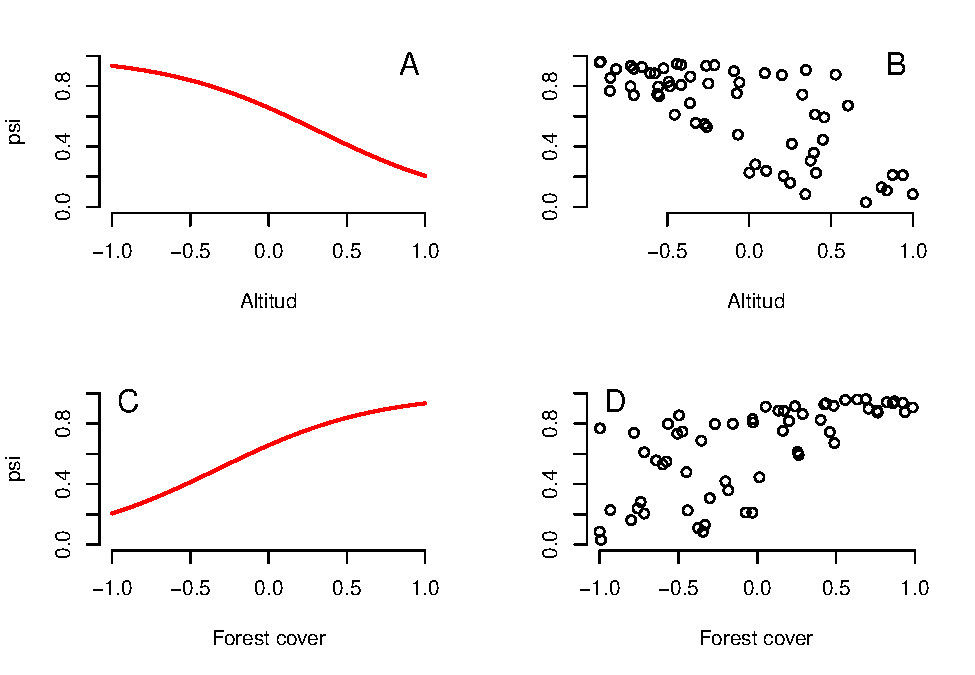
\includegraphics{Simul-Machalilla-book_files/figure-latex/graph2-1.pdf}
\caption{\label{fig:graph2}Dos formas de mostrar la relación entre la
probabilidad de ocurrencia de los venados y las co-variables. (A)
Relación entre psi y altitud para un valor constante (media igual a
cero) de cobertura boscosa. (B) Relación entre psi y la altitud en un
valor observado de cobertura boscosa. (C) relación psi cobertura boscosa
para una altitud constante (en la media de cero). (D) Relación psi
cobertura boscosa para el valor observado de altitud.}
\end{figure}

\begin{Shaded}
\begin{Highlighting}[]
\CommentTok{# dev.off()}
\KeywordTok{par}\NormalTok{(opar)          }\CommentTok{# restore original par settings}
\end{Highlighting}
\end{Shaded}

Para mostrar mejor la relación conjunta entre las dos covariables y psi,
debemos realizar un diagrama de superficie. Aquí no hemos cambiado nada
de la simulación, solo le hemos agregado más datos para visualizar
mejor.

\begin{Shaded}
\begin{Highlighting}[]
\CommentTok{# Compute expected occurrence for a grid of elevation and forest cover}
\NormalTok{cov1 <-}\StringTok{ }\KeywordTok{seq}\NormalTok{(-}\DecValTok{1}\NormalTok{, }\DecValTok{1}\NormalTok{, , }\DecValTok{100}\NormalTok{)                       }\CommentTok{# Values for elevation}
\NormalTok{cov2 <-}\StringTok{ }\KeywordTok{seq}\NormalTok{(-}\DecValTok{1}\NormalTok{, }\DecValTok{1}\NormalTok{, , }\DecValTok{100}\NormalTok{)                       }\CommentTok{# Values for forest cover}
\NormalTok{psi.matrix <-}\StringTok{ }\KeywordTok{array}\NormalTok{(}\OtherTok{NA}\NormalTok{, }\DataTypeTok{dim =} \KeywordTok{c}\NormalTok{(}\DecValTok{100}\NormalTok{, }\DecValTok{100}\NormalTok{))      }\CommentTok{# Prediction matrix, for every }
\CommentTok{# combination of values of elevation and forest cover}

\NormalTok{for(i in }\DecValTok{1}\NormalTok{:}\DecValTok{100}\NormalTok{)\{}
   \NormalTok{for(j in }\DecValTok{1}\NormalTok{:}\DecValTok{100}\NormalTok{)\{}
      \NormalTok{psi.matrix[i, j] <-}\StringTok{ }\KeywordTok{plogis}\NormalTok{(beta0 +}\StringTok{ }
\StringTok{                                   }\NormalTok{beta1 *}\StringTok{ }\NormalTok{cov1[i] +}\StringTok{ }
\StringTok{                                   }\NormalTok{beta2 *}\StringTok{ }\NormalTok{cov2[j] +}\StringTok{ }
\StringTok{                                   }\NormalTok{beta3 *}\StringTok{ }\NormalTok{cov1[i] *}\StringTok{ }\NormalTok{cov2[j] )}
   \NormalTok{\}}
\NormalTok{\}}

\NormalTok{mapPalette <-}\StringTok{ }\KeywordTok{colorRampPalette}\NormalTok{(}\KeywordTok{c}\NormalTok{(}\StringTok{"grey"}\NormalTok{, }\StringTok{"yellow"}\NormalTok{, }\StringTok{"orange"}\NormalTok{, }\StringTok{"red"}\NormalTok{))}
\KeywordTok{image}\NormalTok{(}\DataTypeTok{x =} \NormalTok{cov1, }\DataTypeTok{y =} \NormalTok{cov2, }\DataTypeTok{z =} \NormalTok{psi.matrix, }\DataTypeTok{col =} \KeywordTok{mapPalette}\NormalTok{(}\DecValTok{100}\NormalTok{), }\DataTypeTok{xlab =} \StringTok{"Altitud"}\NormalTok{, }
      \DataTypeTok{ylab =} \StringTok{"Forest cover"}\NormalTok{, }\DataTypeTok{cex.lab =} \FloatTok{1.2}\NormalTok{)}
\KeywordTok{contour}\NormalTok{(}\DataTypeTok{x =} \NormalTok{cov1, }\DataTypeTok{y =} \NormalTok{cov2, }\DataTypeTok{z =} \NormalTok{psi.matrix, }\DataTypeTok{add =} \OtherTok{TRUE}\NormalTok{, }\DataTypeTok{lwd =} \DecValTok{1}\NormalTok{)}
\KeywordTok{matpoints}\NormalTok{(elev, forest, }\DataTypeTok{pch=}\StringTok{"+"}\NormalTok{, }\DataTypeTok{cex=}\FloatTok{0.8}\NormalTok{)}
\end{Highlighting}
\end{Shaded}

\begin{figure}[htbp]
\centering
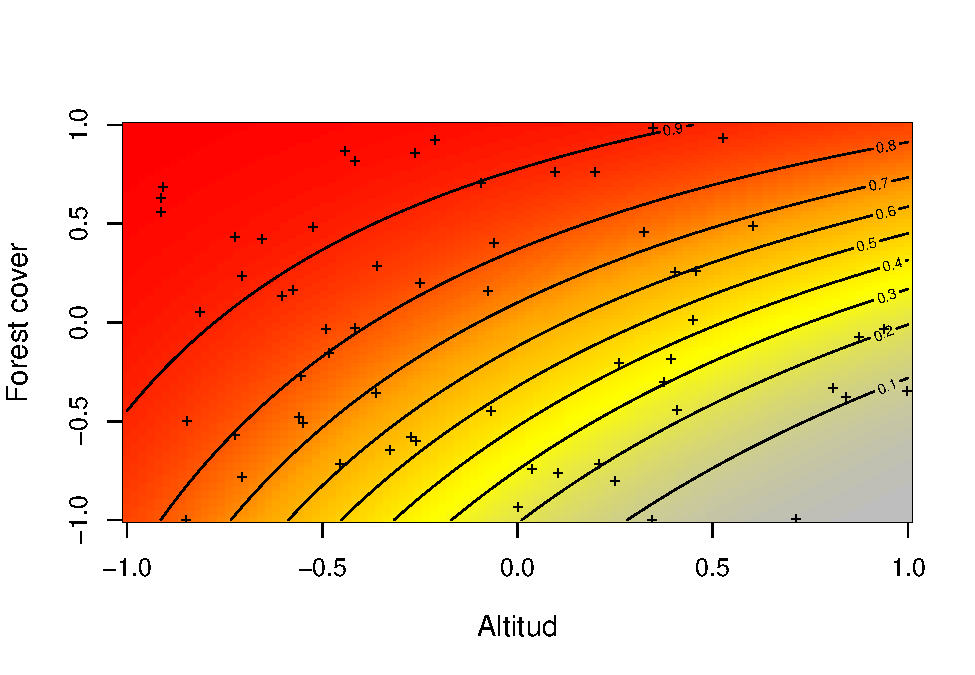
\includegraphics{Simul-Machalilla-book_files/figure-latex/gpagh3-1.pdf}
\caption{\label{fig:gpagh3}Relación construida ente los datos simulados de
la ocurrencia esperada (ocupación) del venado (psi) representada con la
escala de color de gris a rojo, contra la altitud y la cobertura boscosa
simultáneamente. En este caso la interaccion entre las dos covariables
esta dada por el valor de beta3 = 1 que hemos establecido
anteriormente.}
\end{figure}

Hasta ahora no hemos introducido ninguna variación estocástica en la
relación entre la ocurrencia del venado y las covariables. Para hacer
esto debemos hacer uso de algunos modelos estadísticos o distribuciones
estadísticas, para describir la variabilidad al azar alrededor del valor
esperado de psi. La forma típica de introducir esta variación al azar es
obtener la ocurrencia de venados en cada sitio \emph{i}, \(z _{i}\), de
una distribución Bernoulli con los valores esperados (\(\psi _{i}\)).

\subsection{Por que Bernoulli?}\label{por-que-bernoulli}

En el proceso ecologico \(z _{i}\) la ocurrencia del venado esta
representado por una distribución de tipo Bernoulli donde el venado este
presente en un sitio representado como la ocupación \(\psi\) en un sitio
en que esta presente, o no esta presente 1-\(\psi\). La distribución
Bernoulli es un caso especial de la distribución binomial, y su mejor
ejemplo es el lanzamiento de una moneda una sola vez. Si requiere una
explicación más extensa, básica, detallada y con mas ejemplos le
recomiendo visitar
\href{https://es.khanacademy.org/math/probability/statistics-inferential/margin-of-error/v/mean-and-variance-of-bernoulli-distribution-example}{khanacademy.}

\begin{Shaded}
\begin{Highlighting}[]
\NormalTok{z <-}\StringTok{ }\KeywordTok{rbinom}\NormalTok{(}\DataTypeTok{n =} \NormalTok{M, }\DataTypeTok{size =} \DecValTok{1}\NormalTok{, }\DataTypeTok{prob =} \NormalTok{psi)  }\CommentTok{# Realised occurrence. A Bernoulli}
\KeywordTok{sum}\NormalTok{(z)                                    }\CommentTok{# Total number of occupied sites}
\end{Highlighting}
\end{Shaded}

\begin{verbatim}
## [1] 40
\end{verbatim}

\begin{Shaded}
\begin{Highlighting}[]
\KeywordTok{table}\NormalTok{(z)                                  }\CommentTok{# Frequency distribution of deer occurrence}
\end{Highlighting}
\end{Shaded}

\begin{verbatim}
## z
##  0  1 
## 20 40
\end{verbatim}

Aquí hemos creado el resultado del proceso ecológico: ocurrencia
específica para cada sitio \(z _{1}\). Vemos que 23 sitios no están
ocupados y que los restantes 37 si están ocupados.

\section{Simulando el proceso de observación y su resultado: la
detección}\label{simulando-el-proceso-de-observacion-y-su-resultado-la-deteccion}

La ocurrencia \emph{z} no es lo que normalmente vemos, ya que hay un
chance de que fallemos en observar un individuo. De ahí que haya una
medida binaria de error cuando medimos la ocurrencia (lo observamos o no
lo observamos). Nosotros asumimos que podemos hacer únicamente una de
las dos posibles observaciones (si, no), pero pudimos haber perdido la
observación de un venado en algún sitio, entonces la probabilidad de
detección es menor que uno y la medida de error es afectada por la
cobertura de bosque y la temperatura. Hay que tener en cuenta que nunca
vamos a registrar la presencia de un venado cuando en realidad no hay
venados. En otras palabras estamos asumiendo que no tenemos falsos
positivos. Para hacer explícito que tenemos un efecto de interacción
entre dos co variables en nuestros datos, vamos a permitir un efecto de
la interacción en el código, pero ajustado a cero y de esta forma sin
efecto en el modelo que genera los datos. Primero seleccionamos los
valores para \(\alpha _{0}\) hasta \(\alpha _{3}\), donde el primero es
la probabilidad de detección para el venado, en la escala logit, cuando
todas las co variables de la detección tienen un valor de cero. Hemos
escogido el intercepto del modelo de detección y luego lo transformamos
con la función de enlace plogis. Esto no es lo mismo que la probabilidad
de detección media, la cual es más alta en nuestro modelo de simulación,
como veremos más adelante.

\begin{Shaded}
\begin{Highlighting}[]
\NormalTok{mean.detection <-}\StringTok{ }\FloatTok{0.3}            \CommentTok{# Mean expected detection}
\NormalTok{alpha0 <-}\StringTok{ }\KeywordTok{qlogis}\NormalTok{(mean.detection) }\CommentTok{# same on logit scale (intercept)}
\NormalTok{alpha1 <-}\StringTok{ }\NormalTok{-}\DecValTok{1}                     \CommentTok{# Effect (slope) of elevation}
\NormalTok{alpha2 <-}\StringTok{ }\NormalTok{-}\DecValTok{3}                     \CommentTok{# Effect (slope) of temperature}
\NormalTok{alpha3 <-}\StringTok{ }\DecValTok{0}                      \CommentTok{# Interaction effect (slope) of elevevation and temperature}
\end{Highlighting}
\end{Shaded}

Aplicando el modelo lineal, tenemos el logit de la probabilidad de
detección del venado para cada sitio y muestreo, y aplicándole la
transformación inversa (plogis), obtenemos una matriz de las dimensiones
60 por 30 con la probabilidad de detección para cada sitio \emph{i} y
muestreo \emph{j}. Finalmente, graficamos las relaciones para la
probabilidad de detección en los datos.

\begin{Shaded}
\begin{Highlighting}[]
\NormalTok{logit.p <-}\StringTok{ }\NormalTok{alpha0 +}\StringTok{ }\NormalTok{alpha1 *}\StringTok{ }\NormalTok{elev +}\StringTok{ }\NormalTok{alpha2 *}\StringTok{ }\NormalTok{temp +}\StringTok{ }\NormalTok{alpha3 *}\StringTok{ }\NormalTok{elev *}\StringTok{ }\NormalTok{temp}
\NormalTok{p <-}\StringTok{ }\KeywordTok{plogis}\NormalTok{(logit.p)             }\CommentTok{# Inverse link transform }
\KeywordTok{mean}\NormalTok{(p)                          }\CommentTok{# average per-site p is about 0.39}
\end{Highlighting}
\end{Shaded}

\begin{verbatim}
## [1] 0.3928068
\end{verbatim}

\begin{Shaded}
\begin{Highlighting}[]
\KeywordTok{par}\NormalTok{(}\DataTypeTok{mfrow =} \KeywordTok{c}\NormalTok{(}\DecValTok{2}\NormalTok{, }\DecValTok{2}\NormalTok{), }\DataTypeTok{mar =} \KeywordTok{c}\NormalTok{(}\DecValTok{5}\NormalTok{,}\DecValTok{4}\NormalTok{,}\DecValTok{2}\NormalTok{,}\DecValTok{2}\NormalTok{), }\DataTypeTok{cex.main =} \DecValTok{1}\NormalTok{)}
\KeywordTok{curve}\NormalTok{(}\KeywordTok{plogis}\NormalTok{(alpha0 +}\StringTok{ }\NormalTok{alpha1*x), -}\DecValTok{1}\NormalTok{, }\DecValTok{1}\NormalTok{, }\DataTypeTok{col =} \StringTok{"red"}\NormalTok{, }\DataTypeTok{frame.plot =} \OtherTok{FALSE}\NormalTok{, }\DataTypeTok{ylim =} \KeywordTok{c}\NormalTok{(}\DecValTok{0}\NormalTok{, }\FloatTok{1.1}\NormalTok{), }
      \DataTypeTok{xlab =} \StringTok{"Altitud"}\NormalTok{, }\DataTypeTok{ylab =} \StringTok{"p"}\NormalTok{, }\DataTypeTok{lwd =} \DecValTok{2}\NormalTok{)}
\KeywordTok{text}\NormalTok{(-}\FloatTok{0.9}\NormalTok{, }\FloatTok{1.05}\NormalTok{, }\StringTok{"A"}\NormalTok{, }\DataTypeTok{cex =} \FloatTok{1.5}\NormalTok{)}
\KeywordTok{matplot}\NormalTok{(elev, p, }\DataTypeTok{pch =} \StringTok{"*"}\NormalTok{, }\DataTypeTok{frame.plot =} \OtherTok{FALSE}\NormalTok{, }\DataTypeTok{ylim =} \KeywordTok{c}\NormalTok{(}\DecValTok{0}\NormalTok{, }\FloatTok{1.1}\NormalTok{), }\DataTypeTok{xlab =} \StringTok{"Altitud"}\NormalTok{, }
        \DataTypeTok{ylab =} \StringTok{""}\NormalTok{)}
\KeywordTok{text}\NormalTok{(-}\FloatTok{0.9}\NormalTok{, }\FloatTok{1.05}\NormalTok{, }\StringTok{"B"}\NormalTok{, }\DataTypeTok{cex =} \FloatTok{1.5}\NormalTok{)}
\KeywordTok{curve}\NormalTok{(}\KeywordTok{plogis}\NormalTok{(alpha0 +}\StringTok{ }\NormalTok{alpha2*x), -}\DecValTok{1}\NormalTok{, }\DecValTok{1}\NormalTok{, }\DataTypeTok{col =} \StringTok{"red"}\NormalTok{, }\DataTypeTok{frame.plot =} \OtherTok{FALSE}\NormalTok{, }\DataTypeTok{ylim =} \KeywordTok{c}\NormalTok{(}\DecValTok{0}\NormalTok{, }\FloatTok{1.1}\NormalTok{), }
      \DataTypeTok{xlab =} \StringTok{"Temperature"}\NormalTok{, }\DataTypeTok{ylab =} \StringTok{"p"}\NormalTok{, }\DataTypeTok{lwd =} \DecValTok{2}\NormalTok{)}
\KeywordTok{text}\NormalTok{(-}\FloatTok{0.9}\NormalTok{, }\FloatTok{1.05}\NormalTok{, }\StringTok{"C"}\NormalTok{, }\DataTypeTok{cex =} \FloatTok{1.5}\NormalTok{)}
\KeywordTok{matplot}\NormalTok{(temp, p, }\DataTypeTok{pch =} \StringTok{"*"}\NormalTok{, }\DataTypeTok{frame.plot =} \OtherTok{FALSE}\NormalTok{, }\DataTypeTok{ylim =} \KeywordTok{c}\NormalTok{(}\DecValTok{0}\NormalTok{, }\FloatTok{1.1}\NormalTok{), }\DataTypeTok{xlab =} \StringTok{"Temperature"}\NormalTok{, }
        \DataTypeTok{ylab =} \StringTok{"p"}\NormalTok{)}
\KeywordTok{text}\NormalTok{(-}\FloatTok{0.9}\NormalTok{, }\FloatTok{1.05}\NormalTok{, }\StringTok{"D"}\NormalTok{, }\DataTypeTok{cex =} \FloatTok{1.5}\NormalTok{)}
\end{Highlighting}
\end{Shaded}

\begin{figure}[htbp]
\centering
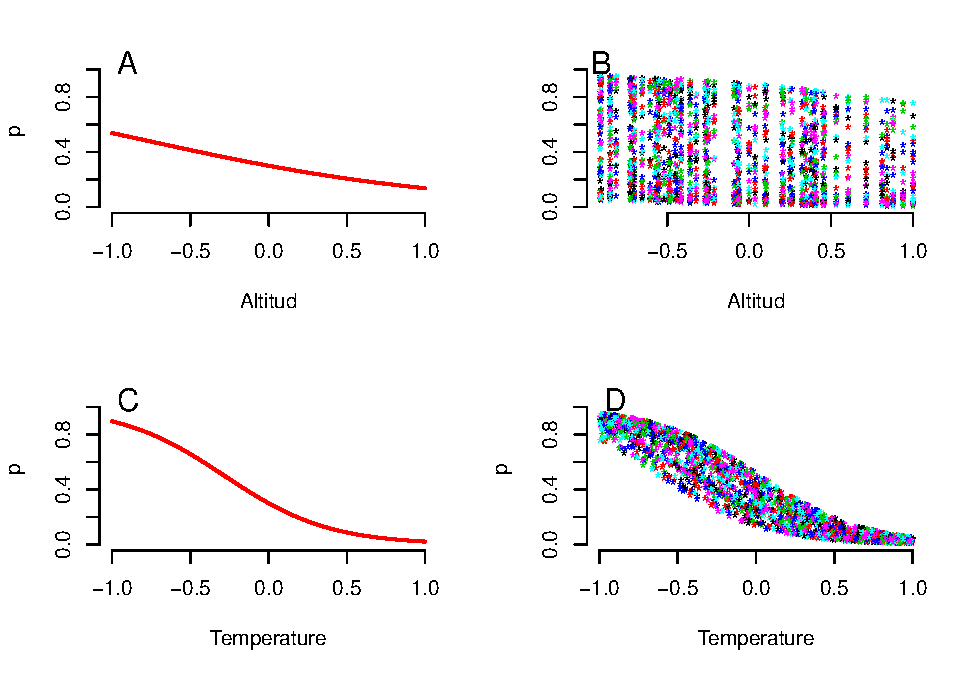
\includegraphics{Simul-Machalilla-book_files/figure-latex/graph4-1.pdf}
\caption{\label{fig:graph4}Dos formas de mostrar las relaciones entre la
probabilidad de detección esperada del venado (\emph{p}) y las dos
variables altitud y temperatura. (A) Relación \emph{p} y altitud para
temperatura constante (en el valor medio, que es igual a cero). (B)
Relación entre \emph{p} y la altitud en el valor observado de cantidad
de temperatura. (C) Relación entre \emph{p} y temperatura para un valor
constante de altitud (en la altitud media igual a cero). (D) Relación
entre \emph{p} y temperatura para un valor observado de altitud.}
\end{figure}

De forma similar vamos a producir una gráfica de una superficie con la
relación conjunta entre la altitud, la temperatura y la probabilidad de
detección del venado (\emph{p}), actuando simultáneamente. La relación
en la escala logarítmica es representada por un plano con pendiente que
representa la interaccion entre la elevacion y la cobertura de bosque.

\begin{Shaded}
\begin{Highlighting}[]
\CommentTok{# Compute expected detection probability for a grid of elevation and temperature}
\NormalTok{cov1 <-}\StringTok{ }\KeywordTok{seq}\NormalTok{(-}\DecValTok{1}\NormalTok{, }\DecValTok{1}\NormalTok{,,}\DecValTok{100}\NormalTok{)                  }\CommentTok{# Values of elevation}
\NormalTok{cov2 <-}\StringTok{ }\KeywordTok{seq}\NormalTok{(-}\DecValTok{1}\NormalTok{,}\DecValTok{1}\NormalTok{,,}\DecValTok{100}\NormalTok{)                   }\CommentTok{# Values of temperature}
\NormalTok{p.matrix <-}\StringTok{ }\KeywordTok{array}\NormalTok{(}\OtherTok{NA}\NormalTok{, }\DataTypeTok{dim =} \KeywordTok{c}\NormalTok{(}\DecValTok{100}\NormalTok{, }\DecValTok{100}\NormalTok{)) }\CommentTok{# Prediction matrix which combines }
\CommentTok{# every value in cov 1 with every other in cov2}
\NormalTok{for(i in }\DecValTok{1}\NormalTok{:}\DecValTok{100}\NormalTok{)\{}
   \NormalTok{for(j in }\DecValTok{1}\NormalTok{:}\DecValTok{100}\NormalTok{)\{}
      \NormalTok{p.matrix[i, j] <-}\StringTok{ }\KeywordTok{plogis}\NormalTok{(alpha0 +}\StringTok{ }\NormalTok{alpha1 *}\StringTok{ }\NormalTok{cov1[i] +}\StringTok{ }
\StringTok{                                 }\NormalTok{alpha2 *}\StringTok{ }\NormalTok{cov2[j] +}\StringTok{ }
\StringTok{                                 }\NormalTok{alpha3 *}\StringTok{ }\NormalTok{cov1[i] *}\StringTok{ }\NormalTok{cov2[j])}
   \NormalTok{\}}
\NormalTok{\}}
\KeywordTok{image}\NormalTok{(}\DataTypeTok{x =} \NormalTok{cov1, }\DataTypeTok{y =} \NormalTok{cov2, }\DataTypeTok{z =} \NormalTok{p.matrix, }\DataTypeTok{col =} \KeywordTok{mapPalette}\NormalTok{(}\DecValTok{100}\NormalTok{), }\DataTypeTok{xlab =} \StringTok{"Altitud"}\NormalTok{, }
      \DataTypeTok{ylab =} \StringTok{"Temperature"}\NormalTok{, }\DataTypeTok{cex.lab =} \FloatTok{1.2}\NormalTok{)}
\KeywordTok{contour}\NormalTok{(}\DataTypeTok{x =} \NormalTok{cov1, }\DataTypeTok{y =} \NormalTok{cov2, }\DataTypeTok{z =} \NormalTok{p.matrix, }\DataTypeTok{add =} \OtherTok{TRUE}\NormalTok{, }\DataTypeTok{lwd =} \DecValTok{1}\NormalTok{)}
\KeywordTok{matpoints}\NormalTok{(elev, temp, }\DataTypeTok{pch=}\StringTok{"+"}\NormalTok{, }\DataTypeTok{cex=}\FloatTok{0.7}\NormalTok{, }\DataTypeTok{col =} \StringTok{"black"}\NormalTok{)}
\end{Highlighting}
\end{Shaded}

\begin{figure}[htbp]
\centering
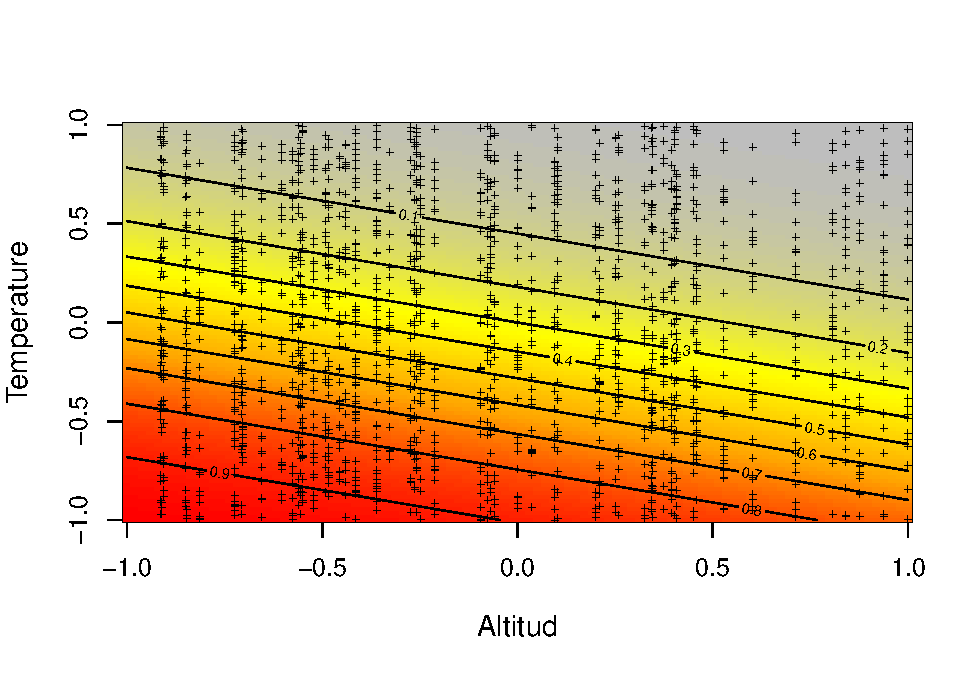
\includegraphics{Simul-Machalilla-book_files/figure-latex/graph5-1.pdf}
\caption{\label{fig:graph5}Relación construida ente los datos simulados de
la probabilidad de deteccion esperada (detectabilidad) del venado (p)
representada con la escala de color de gris a rojo, contra la altitud y
la temperatura simultáneamente. En este caso la interaccion entre las
dos covariables tiene una relacion lineal que esta dada por el valor de
alpha3 = 0 que hemos establecido anteriormente.}
\end{figure}

Hasta aca memos modelado los dos procesos el ecologico \(z\) y el de
observación \emph{p} por aparte. Ahora tendremos que ponerlos juntos, y
para esto multiplicamos el resultado del proceso ecologico por la
probabilidad de deteccion dentro de una distribucion Bernoulli.

\subsection{Uniendo los dos procesos el ecologico y el de
observación}\label{uniendo-los-dos-procesos-el-ecologico-y-el-de-observacion}

Cuando ``medimos'' la ocurrencia, la detección imperfecta, representa
una fuente de error con una distribución de tipo Bernoulli (por ejemplo
la presencia del venado en un sitio en que es detectado con una
probabilidad \emph{p}, o no es detectado como 1-\emph{p}. Al aplicar
este proceso de observación producimos medidas repetidas de la presencia
o ausencia (1 o 0) del venado en cada sitio. Recuerde que la
distribución Bernoulli es un caso especial de la distribución binomial,
y su mejor ejemplo es el lanzamiento de una moneda una sola vez.

En este momento estamos estableciendo la jerarquia en el modelo
jerarquico. Aca estamos anidando el proceso ecologico ``dentro'' del
proceso de observación.

\begin{Shaded}
\begin{Highlighting}[]
\NormalTok{y <-}\StringTok{ }\KeywordTok{matrix}\NormalTok{(}\OtherTok{NA}\NormalTok{, }\DataTypeTok{nrow =} \NormalTok{M, }\DataTypeTok{ncol =} \NormalTok{J)      }\CommentTok{# Prepare array for counts}
\NormalTok{for (i in }\DecValTok{1}\NormalTok{:J)\{                          }\CommentTok{# Generate counts}
   \NormalTok{y[,i] <-}\StringTok{ }\KeywordTok{rbinom}\NormalTok{(}\DataTypeTok{n =} \NormalTok{M, }\DataTypeTok{size =} \DecValTok{1}\NormalTok{, }\DataTypeTok{prob =} \NormalTok{z*p[,i])   }\CommentTok{# this is the Bernoulli}
\NormalTok{\}}
\end{Highlighting}
\end{Shaded}

Hasta acá hemos simulado la presencia/ausencia del venado de cola blanca
en 60 sitios durante 30 sesiones de muestreo. Veamos que contienen las
tablas. Recuerde que los sitios están en las filas y los muestreos
repetidos en las columnas. Para comparar, mostraremos la verdadera
ocurrencia en la primera columna para 30 sitios y solo cinco muestreos.

\begin{Shaded}
\begin{Highlighting}[]
\KeywordTok{library}\NormalTok{(knitr)}
\KeywordTok{kable}\NormalTok{(}\KeywordTok{as.data.frame}\NormalTok{(}\KeywordTok{head}\NormalTok{(}\KeywordTok{cbind}\NormalTok{(}\StringTok{"True Presence/Absence"} \NormalTok{=}\StringTok{ }\NormalTok{z, }
           \StringTok{"1st survey"} \NormalTok{=}\StringTok{ }\NormalTok{y[,}\DecValTok{1}\NormalTok{], }
           \StringTok{"2nd survey"} \NormalTok{=}\StringTok{ }\NormalTok{y[,}\DecValTok{2}\NormalTok{], }
           \StringTok{"3rd survey"} \NormalTok{=}\StringTok{ }\NormalTok{y[,}\DecValTok{3}\NormalTok{],}
           \StringTok{"4th survey"} \NormalTok{=}\StringTok{ }\NormalTok{y[,}\DecValTok{4}\NormalTok{],}
           \StringTok{"5th survey"} \NormalTok{=}\StringTok{ }\NormalTok{y[,}\DecValTok{5}\NormalTok{]), }\DecValTok{30}\NormalTok{)) )   }\CommentTok{# First 30 rows (= sites)}
\end{Highlighting}
\end{Shaded}

\begin{tabular}{r|r|r|r|r|r}
\hline
True Presence/Absence & 1st survey & 2nd survey & 3rd survey & 4th survey & 5th survey\\
\hline
1 & 0 & 1 & 0 & 1 & 0\\
\hline
1 & 0 & 0 & 0 & 1 & 1\\
\hline
1 & 0 & 1 & 0 & 1 & 0\\
\hline
0 & 0 & 0 & 0 & 0 & 0\\
\hline
1 & 1 & 1 & 1 & 0 & 0\\
\hline
1 & 0 & 1 & 0 & 0 & 0\\
\hline
1 & 0 & 0 & 1 & 0 & 1\\
\hline
0 & 0 & 0 & 0 & 0 & 0\\
\hline
1 & 0 & 0 & 0 & 1 & 1\\
\hline
1 & 1 & 0 & 0 & 0 & 0\\
\hline
0 & 0 & 0 & 0 & 0 & 0\\
\hline
0 & 0 & 0 & 0 & 0 & 0\\
\hline
0 & 0 & 0 & 0 & 0 & 0\\
\hline
1 & 0 & 0 & 0 & 0 & 0\\
\hline
1 & 1 & 0 & 0 & 0 & 0\\
\hline
0 & 0 & 0 & 0 & 0 & 0\\
\hline
1 & 0 & 0 & 1 & 1 & 0\\
\hline
1 & 1 & 1 & 1 & 1 & 0\\
\hline
0 & 0 & 0 & 0 & 0 & 0\\
\hline
1 & 0 & 0 & 0 & 1 & 1\\
\hline
1 & 1 & 1 & 1 & 1 & 0\\
\hline
0 & 0 & 0 & 0 & 0 & 0\\
\hline
0 & 0 & 0 & 0 & 0 & 0\\
\hline
1 & 1 & 0 & 0 & 0 & 1\\
\hline
1 & 0 & 0 & 0 & 1 & 1\\
\hline
0 & 0 & 0 & 0 & 0 & 0\\
\hline
1 & 1 & 1 & 0 & 1 & 0\\
\hline
1 & 0 & 1 & 1 & 0 & 0\\
\hline
1 & 1 & 1 & 0 & 0 & 0\\
\hline
1 & 0 & 1 & 0 & 0 & 1\\
\hline
\end{tabular}

Ahora finalmente visualizaremos graficamente los datos de unos y ceros
que hemos simulado para nuestro muestreo. Recuerde que se trata de
valores de unos que representan si hemos detectado, o no hemos detectado
al venado, en cada uno de los sitios de muestreo en cada una de las
visitas.

\begin{Shaded}
\begin{Highlighting}[]
\KeywordTok{par}\NormalTok{(}\DataTypeTok{mfrow =} \KeywordTok{c}\NormalTok{(}\DecValTok{2}\NormalTok{, }\DecValTok{2}\NormalTok{), }\DataTypeTok{mar =} \KeywordTok{c}\NormalTok{(}\DecValTok{5}\NormalTok{,}\DecValTok{4}\NormalTok{,}\DecValTok{2}\NormalTok{,}\DecValTok{2}\NormalTok{), }\DataTypeTok{cex.main =} \DecValTok{1}\NormalTok{)}
\KeywordTok{matplot}\NormalTok{(elev, }\KeywordTok{jitter}\NormalTok{(y), }\DataTypeTok{pch =} \StringTok{"*"}\NormalTok{, }\DataTypeTok{frame.plot =} \OtherTok{FALSE}\NormalTok{, }\DataTypeTok{ylim =} \KeywordTok{c}\NormalTok{(}\DecValTok{0}\NormalTok{, }\DecValTok{1}\NormalTok{), }
        \DataTypeTok{xlab =} \StringTok{"Altitud"}\NormalTok{, }\DataTypeTok{ylab =} \StringTok{"Detection/Nondetection (y)"}\NormalTok{)}
\KeywordTok{matplot}\NormalTok{(forest, }\KeywordTok{jitter}\NormalTok{(y), }\DataTypeTok{pch =} \StringTok{"*"}\NormalTok{, }\DataTypeTok{frame.plot =} \OtherTok{FALSE}\NormalTok{, }\DataTypeTok{ylim =} \KeywordTok{c}\NormalTok{(}\DecValTok{0}\NormalTok{, }\DecValTok{1}\NormalTok{), }
        \DataTypeTok{xlab =} \StringTok{"Forest cover"}\NormalTok{, }\DataTypeTok{ylab =} \StringTok{"Detection/Nondetection (y)"}\NormalTok{)}
\KeywordTok{matplot}\NormalTok{(temp, }\KeywordTok{jitter}\NormalTok{(y), }\DataTypeTok{pch =} \StringTok{"*"}\NormalTok{, }\DataTypeTok{frame.plot =} \OtherTok{FALSE}\NormalTok{, }\DataTypeTok{ylim =} \KeywordTok{c}\NormalTok{(}\DecValTok{0}\NormalTok{, }\DecValTok{1}\NormalTok{), }
        \DataTypeTok{xlab =} \StringTok{"Teperature"}\NormalTok{, }\DataTypeTok{ylab =} \StringTok{"Detection/Nondetection (y)"}\NormalTok{)}
\KeywordTok{hist}\NormalTok{(y, }\DataTypeTok{breaks =} \DecValTok{50}\NormalTok{, }\DataTypeTok{col =} \StringTok{"grey"}\NormalTok{, }\DataTypeTok{ylim =} \KeywordTok{c}\NormalTok{(}\DecValTok{0}\NormalTok{, }\DecValTok{600}\NormalTok{), }\DataTypeTok{main =} \StringTok{""}\NormalTok{, }
     \DataTypeTok{xlab =} \StringTok{"Detection/Nondetection (y)"}\NormalTok{)}
\end{Highlighting}
\end{Shaded}

\begin{figure}[htbp]
\centering
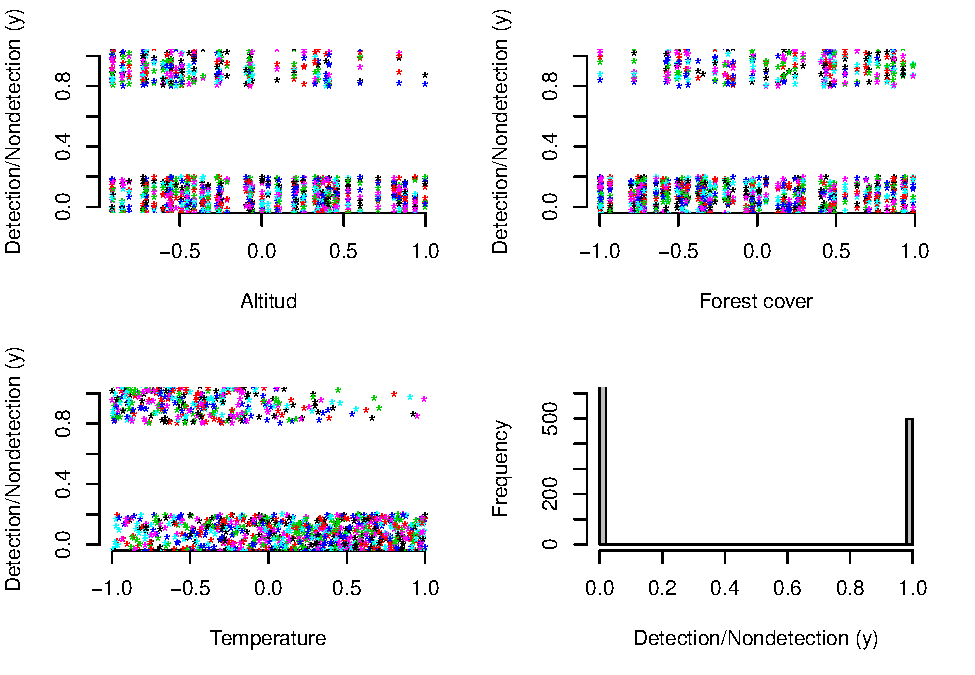
\includegraphics{Simul-Machalilla-book_files/figure-latex/graph6-1.pdf}
\caption{\label{fig:graph6}Relación entre la (jittered) ocupación observada
de venados (y) y las tres covariables estandarizadas. Altitud (A).
Cobertura de bosque (B). Temperatura (C) y la frecuencia de distribución
de la ocurrencia observada (y) en un set de datos de 60 sitios con 30
muestreos cada uno (D).}
\end{figure}

Hasta aquí hemos creado un set de datos donde la detección/no detección
del venado esta negativamente correlacionado con la temperatura y
positivamente relacionado con la cobertura de bosque. Hay una razón por
la cual esta correlación entre variables es diferente. La ocurrencia por
sitio, el objetivo de la inferencia ecológica, está afectado por la
cobertura de bosque y la altitud, pero no por la temperatura, mientras
que la probabilidad de detección, el parámetro caracterizando la medida
del proceso de error cuando tomamos medidas de ocurrencia, es también
afectado por la altitud y adicionalmente por la temperatura. Por lo
tanto, como se puede notar, hay un gran reto para poder desenredar la
razón de la variación espacio-temporal en la observación de los datos de
detección/no detección, dado que pueden ser afectados por dos procesos
totalmente diferentes: el ecológico y el observacional, que tambien la
misma covariable puede afectar los dos procesos y que tambien pueden
existir interacciones entre covariables.

\chapter{Empacando todo en una función}\label{function1}

Podría ser de mucha utilidad empacar todo lo que hemos hecho en una sola
función que nos permita hacer lo mismo muchas veces repetidamente. Esto
hará que podamos diseñar simulaciones de una forma más concisa y
flexible y hace mas transparente la generación de parámetros usados para
generar datos. Asi que vamos a definir una función (que llamaremos
data.fn) para generar el mismo tipo de datos que acabamos de crear,
asignando argumentos a la función, tales como tamaño de la muestra,
efectos de las covariables y direcciones y magnitudes de la interacción
de los términos del error de detección y ocupación. Esto hará que
nuestro código sea más flexible y eficiente.

\begin{Shaded}
\begin{Highlighting}[]
\NormalTok{###############################}
\NormalTok{## The function starts here ###}
\NormalTok{###############################}

\CommentTok{# Function definition with set of default values}
\NormalTok{data.fn <-}\StringTok{ }\NormalTok{function(}\DataTypeTok{M =} \DecValTok{60}\NormalTok{, }\DataTypeTok{J =} \DecValTok{30}\NormalTok{, }\DataTypeTok{mean.occupancy =} \FloatTok{0.6}\NormalTok{, }
                    \DataTypeTok{beta1 =} \NormalTok{-}\DecValTok{2}\NormalTok{, }\DataTypeTok{beta2 =} \DecValTok{2}\NormalTok{, }\DataTypeTok{beta3 =} \DecValTok{1}\NormalTok{, }\DataTypeTok{mean.detection =} \FloatTok{0.3}\NormalTok{, }
                    \DataTypeTok{alpha1 =} \NormalTok{-}\DecValTok{1}\NormalTok{, }\DataTypeTok{alpha2 =} \NormalTok{-}\DecValTok{3}\NormalTok{, }\DataTypeTok{alpha3 =} \DecValTok{0}\NormalTok{, }\DataTypeTok{show.plot =} \OtherTok{TRUE}\NormalTok{)\{}
\CommentTok{# Function to simulate occupancy measurements replicated at M sites during J occasions.}
\CommentTok{# Population closure is assumed for each site.}
\CommentTok{# Expected occurrence may be affected by elevation (elev), }
\CommentTok{# forest cover (forest) and their interaction.}
\CommentTok{# Expected detection probability may be affected by elevation, }
\CommentTok{# temperature (temp) and their interaction.}
\CommentTok{# Function arguments:}
\CommentTok{#     M: Number of spatial replicates (sites)}
\CommentTok{#     J: Number of temporal replicates (occasions)}
\CommentTok{#     mean.occupancy: Mean occurrence at value 0 of occurrence covariates}
\CommentTok{#     beta1: Main effect of elevation on occurrence}
\CommentTok{#     beta2: Main effect of forest cover on occurrence}
\CommentTok{#     beta3: Interaction effect on occurrence of elevation and forest cover}
\CommentTok{#     mean.detection: Mean detection prob. at value 0 of detection covariates}
\CommentTok{#     alpha1: Main effect of elevation on detection probability}
\CommentTok{#     alpha2: Main effect of temperature on detection probability}
\CommentTok{#     alpha3: Interaction effect on detection of elevation and temperature}
\CommentTok{#     show.plot: if TRUE, plots of the data will be displayed; }
\CommentTok{#               set to FALSE if you are running simulations.}

\CommentTok{# Create covariates}
\NormalTok{elev <-}\StringTok{ }\KeywordTok{runif}\NormalTok{(}\DataTypeTok{n =} \NormalTok{M, -}\DecValTok{1}\NormalTok{, }\DecValTok{1}\NormalTok{)                         }\CommentTok{# Scaled elevation}
\NormalTok{forest <-}\StringTok{ }\KeywordTok{runif}\NormalTok{(}\DataTypeTok{n =} \NormalTok{M, -}\DecValTok{1}\NormalTok{, }\DecValTok{1}\NormalTok{)                       }\CommentTok{# Scaled forest cover}
\NormalTok{temp <-}\StringTok{ }\KeywordTok{array}\NormalTok{(}\KeywordTok{runif}\NormalTok{(}\DataTypeTok{n =} \NormalTok{M*J, -}\DecValTok{1}\NormalTok{, }\DecValTok{1}\NormalTok{), }\DataTypeTok{dim =} \KeywordTok{c}\NormalTok{(M, J)) }\CommentTok{# Scaled temperature}

\CommentTok{# Model for occurrence}
\NormalTok{beta0 <-}\StringTok{ }\KeywordTok{qlogis}\NormalTok{(mean.occupancy)               }\CommentTok{# Mean occurrence on link scale}
\NormalTok{psi <-}\StringTok{ }\KeywordTok{plogis}\NormalTok{(beta0 +}\StringTok{ }\NormalTok{beta1*elev +}\StringTok{ }\NormalTok{beta2*forest +}\StringTok{ }\NormalTok{beta3*elev*forest)}
\NormalTok{z <-}\StringTok{ }\KeywordTok{rbinom}\NormalTok{(}\DataTypeTok{n =} \NormalTok{M, }\DataTypeTok{size =} \DecValTok{1}\NormalTok{, }\DataTypeTok{prob =} \NormalTok{psi)      }\CommentTok{# Realised occurrence}

\CommentTok{# Plots}
\NormalTok{if(show.plot)\{}
  \KeywordTok{par}\NormalTok{(}\DataTypeTok{mfrow =} \KeywordTok{c}\NormalTok{(}\DecValTok{2}\NormalTok{, }\DecValTok{2}\NormalTok{), }\DataTypeTok{cex.main =} \DecValTok{1}\NormalTok{)}
  \KeywordTok{devAskNewPage}\NormalTok{(}\DataTypeTok{ask =} \OtherTok{TRUE}\NormalTok{)}
  \KeywordTok{curve}\NormalTok{(}\KeywordTok{plogis}\NormalTok{(beta0 +}\StringTok{ }\NormalTok{beta1*x), -}\DecValTok{1}\NormalTok{, }\DecValTok{1}\NormalTok{, }\DataTypeTok{col =} \StringTok{"red"}\NormalTok{, }\DataTypeTok{frame.plot =} \OtherTok{FALSE}\NormalTok{, }
      \DataTypeTok{ylim =} \KeywordTok{c}\NormalTok{(}\DecValTok{0}\NormalTok{, }\DecValTok{1}\NormalTok{), }\DataTypeTok{xlab =} \StringTok{"Elevation"}\NormalTok{, }\DataTypeTok{ylab =} \StringTok{"psi"}\NormalTok{, }\DataTypeTok{lwd =} \DecValTok{2}\NormalTok{)}
  \KeywordTok{plot}\NormalTok{(elev, psi, }\DataTypeTok{frame.plot =} \OtherTok{FALSE}\NormalTok{, }\DataTypeTok{ylim =} \KeywordTok{c}\NormalTok{(}\DecValTok{0}\NormalTok{, }\DecValTok{1}\NormalTok{), }\DataTypeTok{xlab =} \StringTok{"Elevation"}\NormalTok{, }
     \DataTypeTok{ylab =} \StringTok{""}\NormalTok{)}
  \KeywordTok{curve}\NormalTok{(}\KeywordTok{plogis}\NormalTok{(beta0 +}\StringTok{ }\NormalTok{beta2*x), -}\DecValTok{1}\NormalTok{, }\DecValTok{1}\NormalTok{, }\DataTypeTok{col =} \StringTok{"red"}\NormalTok{, }\DataTypeTok{frame.plot =} \OtherTok{FALSE}\NormalTok{, }
      \DataTypeTok{ylim =} \KeywordTok{c}\NormalTok{(}\DecValTok{0}\NormalTok{, }\DecValTok{1}\NormalTok{), }\DataTypeTok{xlab =} \StringTok{"Forest cover"}\NormalTok{, }\DataTypeTok{ylab =} \StringTok{"psi"}\NormalTok{, }\DataTypeTok{lwd =} \DecValTok{2}\NormalTok{)}
  \KeywordTok{plot}\NormalTok{(forest, psi, }\DataTypeTok{frame.plot =} \OtherTok{FALSE}\NormalTok{, }\DataTypeTok{ylim =} \KeywordTok{c}\NormalTok{(}\DecValTok{0}\NormalTok{, }\DecValTok{1}\NormalTok{), }\DataTypeTok{xlab =} \StringTok{"Forest cover"}\NormalTok{, }
     \DataTypeTok{ylab =} \StringTok{""}\NormalTok{)}
\NormalTok{\}}

\CommentTok{# Model for observations}
\NormalTok{y <-}\StringTok{ }\NormalTok{p <-}\StringTok{ }\KeywordTok{matrix}\NormalTok{(}\OtherTok{NA}\NormalTok{, }\DataTypeTok{nrow =} \NormalTok{M, }\DataTypeTok{ncol =} \NormalTok{J)}\CommentTok{# Prepare matrix for y and p}
\NormalTok{alpha0 <-}\StringTok{ }\KeywordTok{qlogis}\NormalTok{(mean.detection)        }\CommentTok{# mean detection on link scale}
\NormalTok{for (j in }\DecValTok{1}\NormalTok{:J)\{                         }\CommentTok{# Generate counts by survey}
   \NormalTok{p[,j] <-}\StringTok{ }\KeywordTok{plogis}\NormalTok{(alpha0 +}\StringTok{ }\NormalTok{alpha1*elev +}\StringTok{ }\NormalTok{alpha2*temp[,j] +}\StringTok{ }\NormalTok{alpha3*elev*temp[,j])}
   \NormalTok{y[,j] <-}\StringTok{ }\KeywordTok{rbinom}\NormalTok{(}\DataTypeTok{n =} \NormalTok{M, }\DataTypeTok{size =} \DecValTok{1}\NormalTok{, }\DataTypeTok{prob =} \NormalTok{z *}\StringTok{ }\NormalTok{p[,j])}
\NormalTok{\}}

\CommentTok{# True and observed measures of 'distribution'}
\NormalTok{sumZ <-}\StringTok{ }\KeywordTok{sum}\NormalTok{(z)                     }\CommentTok{# Total occurrence (all sites)}
\NormalTok{sumZ.obs <-}\StringTok{ }\KeywordTok{sum}\NormalTok{(}\KeywordTok{apply}\NormalTok{(y,}\DecValTok{1}\NormalTok{,max))    }\CommentTok{# Observed number of occ sites}
\NormalTok{psi.fs.true <-}\StringTok{ }\KeywordTok{sum}\NormalTok{(z) /}\StringTok{ }\NormalTok{M          }\CommentTok{# True proportion of occ. sites in sample}
\NormalTok{psi.fs.obs <-}\StringTok{ }\KeywordTok{mean}\NormalTok{(}\KeywordTok{apply}\NormalTok{(y,}\DecValTok{1}\NormalTok{,max)) }\CommentTok{# Observed proportion of occ. sites in sample}

\CommentTok{# More plots}
\NormalTok{if(show.plot)\{}
  \KeywordTok{par}\NormalTok{(}\DataTypeTok{mfrow =} \KeywordTok{c}\NormalTok{(}\DecValTok{2}\NormalTok{, }\DecValTok{2}\NormalTok{))}
  \KeywordTok{curve}\NormalTok{(}\KeywordTok{plogis}\NormalTok{(alpha0 +}\StringTok{ }\NormalTok{alpha1*x), -}\DecValTok{1}\NormalTok{, }\DecValTok{1}\NormalTok{, }\DataTypeTok{col =} \StringTok{"red"}\NormalTok{, }
      \DataTypeTok{main =} \StringTok{"Relationship p-elevation }\CharTok{\textbackslash{}n}\StringTok{at average temperature"}\NormalTok{, }
      \DataTypeTok{xlab =} \StringTok{"Scaled elevation"}\NormalTok{, }\DataTypeTok{frame.plot =} \NormalTok{F)}
  \KeywordTok{matplot}\NormalTok{(elev, p, }\DataTypeTok{xlab =} \StringTok{"Scaled elevation"}\NormalTok{, }
        \DataTypeTok{main =} \StringTok{"Relationship p-elevation}\CharTok{\textbackslash{}n}\StringTok{ at observed temperature"}\NormalTok{, }
        \DataTypeTok{pch =} \StringTok{"*"}\NormalTok{, }\DataTypeTok{frame.plot =} \NormalTok{F)}
  \KeywordTok{curve}\NormalTok{(}\KeywordTok{plogis}\NormalTok{(alpha0 +}\StringTok{ }\NormalTok{alpha2*x), -}\DecValTok{1}\NormalTok{, }\DecValTok{1}\NormalTok{, }\DataTypeTok{col =} \StringTok{"red"}\NormalTok{, }
      \DataTypeTok{main =} \StringTok{"Relationship p-temperature }\CharTok{\textbackslash{}n}\StringTok{ at average elevation"}\NormalTok{, }
      \DataTypeTok{xlab =} \StringTok{"Scaled temperature"}\NormalTok{, }\DataTypeTok{frame.plot =} \NormalTok{F)}
  \KeywordTok{matplot}\NormalTok{(temp, p, }\DataTypeTok{xlab =} \StringTok{"Scaled temperature"}\NormalTok{, }
        \DataTypeTok{main =} \StringTok{"Relationship p-temperature }\CharTok{\textbackslash{}n}\StringTok{at observed elevation"}\NormalTok{, }
        \DataTypeTok{pch =} \StringTok{"*"}\NormalTok{, }\DataTypeTok{frame.plot =} \NormalTok{F)}
\NormalTok{\}}

\CommentTok{# Output}
\KeywordTok{return}\NormalTok{(}\KeywordTok{list}\NormalTok{(}\DataTypeTok{M =} \NormalTok{M, }\DataTypeTok{J =} \NormalTok{J, }\DataTypeTok{mean.occupancy =} \NormalTok{mean.occupancy, }
            \DataTypeTok{beta0 =} \NormalTok{beta0, }\DataTypeTok{beta1 =} \NormalTok{beta1, }\DataTypeTok{beta2 =} \NormalTok{beta2, }\DataTypeTok{beta3 =} \NormalTok{beta3, }
            \DataTypeTok{mean.detection =} \NormalTok{mean.detection, }
            \DataTypeTok{alpha0 =} \NormalTok{alpha0, }\DataTypeTok{alpha1 =} \NormalTok{alpha1, }\DataTypeTok{alpha2 =} \NormalTok{alpha2, }\DataTypeTok{alpha3 =} \NormalTok{alpha3, }
            \DataTypeTok{elev =} \NormalTok{elev, }\DataTypeTok{forest =} \NormalTok{forest, }\DataTypeTok{temp =} \NormalTok{temp, }
            \DataTypeTok{psi =} \NormalTok{psi, }\DataTypeTok{z =} \NormalTok{z, }\DataTypeTok{p =} \NormalTok{p, }\DataTypeTok{y =} \NormalTok{y, }\DataTypeTok{sumZ =} \NormalTok{sumZ, }\DataTypeTok{sumZ.obs =} \NormalTok{sumZ.obs, }
            \DataTypeTok{psi.fs.true =} \NormalTok{psi.fs.true, }\DataTypeTok{psi.fs.obs =} \NormalTok{psi.fs.obs))}
\NormalTok{\}}

\NormalTok{###############################}
\NormalTok{## The function ends  here  ###}
\NormalTok{###############################}
\end{Highlighting}
\end{Shaded}

Una vez que hayamos definido la función y ejecutado su código, podremos
llamarla repetidamente y enviar los resultados a la pantalla o
asignarlos a un objeto en R. De forma tal que podamos usar el set de
datos almacenado en el objeto para un análisis detallado.

\begin{Shaded}
\begin{Highlighting}[]
\KeywordTok{data.fn}\NormalTok{()                  }\CommentTok{# Execute function with default arguments}
\KeywordTok{data.fn}\NormalTok{(}\DataTypeTok{show.plot =} \OtherTok{FALSE}\NormalTok{) }\CommentTok{# same, without plots}
\NormalTok{objeto1 <-}\StringTok{ }\KeywordTok{data.fn}\NormalTok{(}\DataTypeTok{M =} \DecValTok{30}\NormalTok{, }\DataTypeTok{J =} \DecValTok{10}\NormalTok{, }\DataTypeTok{mean.occupancy =} \FloatTok{0.5}\NormalTok{, }
                   \DataTypeTok{beta1 =} \NormalTok{-}\DecValTok{2}\NormalTok{, }\DataTypeTok{beta2 =} \DecValTok{2}\NormalTok{, }\DataTypeTok{beta3 =} \DecValTok{1}\NormalTok{, }
                   \DataTypeTok{mean.detection =} \FloatTok{0.25}\NormalTok{, }\DataTypeTok{alpha1 =} \NormalTok{-}\DecValTok{1}\NormalTok{,}
                   \DataTypeTok{alpha2 =} \NormalTok{-}\DecValTok{3}\NormalTok{, }\DataTypeTok{alpha3 =} \DecValTok{0}\NormalTok{, }\DataTypeTok{show.plot =} \OtherTok{TRUE}\NormalTok{) }\CommentTok{# Explicit defaults}
\end{Highlighting}
\end{Shaded}

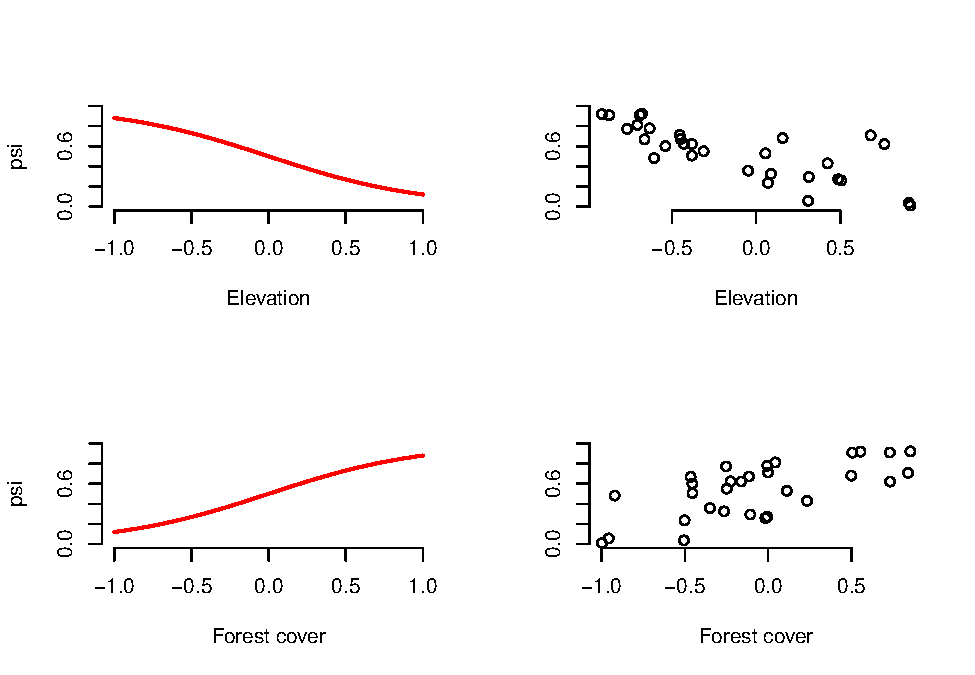
\includegraphics{Simul-Machalilla-book_files/figure-latex/funcall1b-1.pdf}
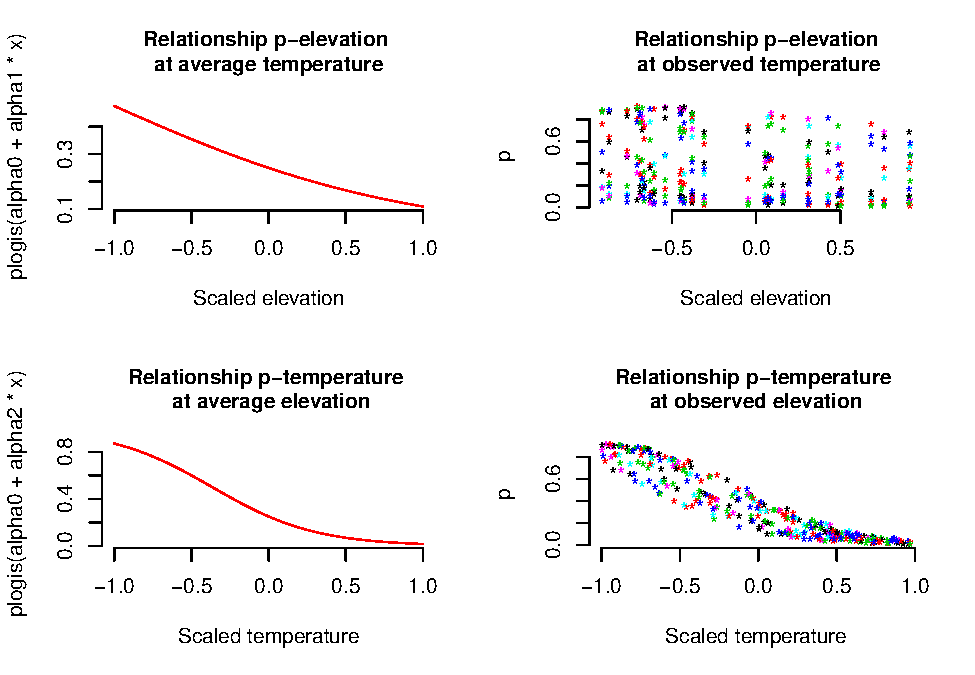
\includegraphics{Simul-Machalilla-book_files/figure-latex/funcall1b-2.pdf}

Tal vez el uso más sencillo posible para esta función es experimentar de
primera mano el error de muestreo: el cuál es la variabilidad natural de
realizaciones repetidas (varios sets de datos) de nuestro proceso
estocástico por el cual calculamos los set de datos. Vamos a simular
10.000 sets de datos del venado para ver como varían en términos del
verdadero número de sitios ocupados (sumZ en el codigo) y el número de
sitios en los que los venados fueron observados al menos una vez.

\begin{Shaded}
\begin{Highlighting}[]
\NormalTok{simrep <-}\StringTok{ }\DecValTok{10000}
\NormalTok{trueSumZ <-}\StringTok{ }\NormalTok{obsSumZ <-}\StringTok{ }\KeywordTok{numeric}\NormalTok{(simrep)}
\NormalTok{for(i in }\DecValTok{1}\NormalTok{:simrep)\{}
   \NormalTok{if(i %%}\StringTok{ }\DecValTok{1000} \NormalTok{==}\DecValTok{0} \NormalTok{)                        }\CommentTok{# report progress}
   \KeywordTok{cat}\NormalTok{(}\StringTok{"iter"}\NormalTok{, i, }\StringTok{"}\CharTok{\textbackslash{}n}\StringTok{"}\NormalTok{)}
   \NormalTok{data <-}\StringTok{ }\KeywordTok{data.fn}\NormalTok{(}\DataTypeTok{M =} \DecValTok{60}\NormalTok{,}\DataTypeTok{J =} \DecValTok{3}\NormalTok{,}\DataTypeTok{show.plot =} \OtherTok{FALSE}\NormalTok{) }\CommentTok{# 60 sitios, 3 muestreos}
   \NormalTok{trueSumZ[i] <-}\StringTok{ }\NormalTok{data$sumZ}
   \NormalTok{obsSumZ[i] <-}\StringTok{ }\KeywordTok{sum}\NormalTok{(}\KeywordTok{apply}\NormalTok{(data$y, }\DecValTok{1}\NormalTok{, max))}
\NormalTok{\}}
\end{Highlighting}
\end{Shaded}

\begin{verbatim}
## iter 1000 
## iter 2000 
## iter 3000 
## iter 4000 
## iter 5000 
## iter 6000 
## iter 7000 
## iter 8000 
## iter 9000 
## iter 10000
\end{verbatim}

\begin{Shaded}
\begin{Highlighting}[]
\KeywordTok{plot}\NormalTok{(}\KeywordTok{sort}\NormalTok{(trueSumZ), }\DataTypeTok{ylim =} \KeywordTok{c}\NormalTok{(}\KeywordTok{min}\NormalTok{(obsSumZ), }\KeywordTok{max}\NormalTok{(trueSumZ)), }\DataTypeTok{ylab =} \StringTok{""}\NormalTok{, }\DataTypeTok{xlab =} \StringTok{"Simulation"}\NormalTok{,}
     \DataTypeTok{col =} \StringTok{"red"}\NormalTok{, }\DataTypeTok{main =} \StringTok{"True (red) and observed (blue) number of occupied sites"}\NormalTok{)}
\KeywordTok{points}\NormalTok{(obsSumZ[}\KeywordTok{order}\NormalTok{(trueSumZ)], }\DataTypeTok{col =} \StringTok{"blue"}\NormalTok{)}
\end{Highlighting}
\end{Shaded}

\begin{figure}[htbp]
\centering
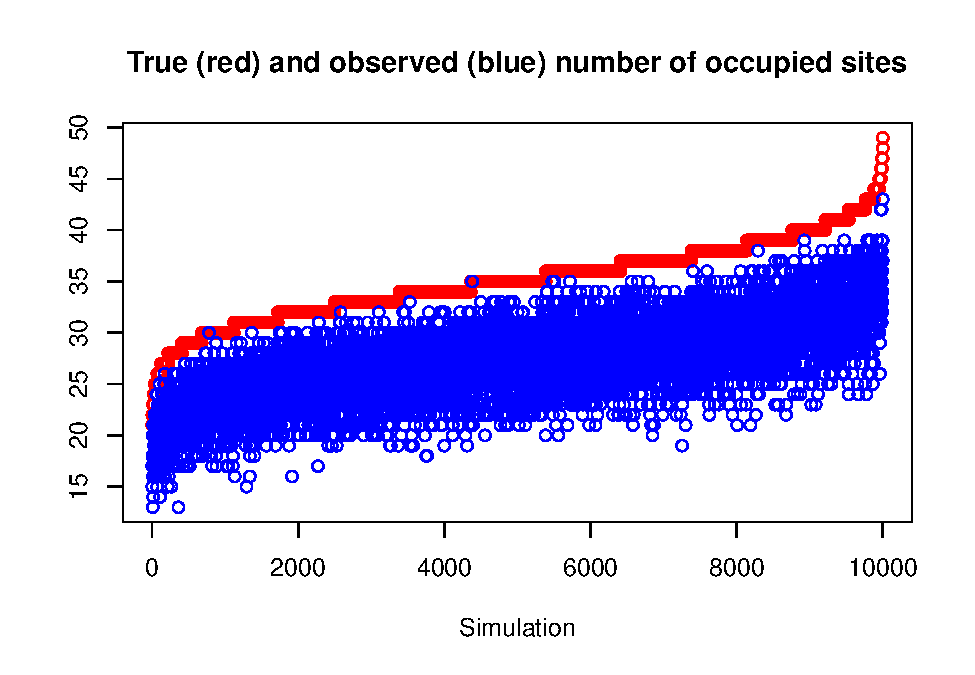
\includegraphics{Simul-Machalilla-book_files/figure-latex/funcall2-1.pdf}
\caption{\label{fig:funcall2}Variabilidad natural (error de muestreo) del
verdadero número de sitios ocupados (ordenados por tamaño) en color rojo
y el número observado de sitios ocupados (en azul), para un muestreo
simulado de venados. El número de sitios observados también se conoce
como la ocupación ingenua o detección ``naïve'' (observable) de la
ocurrencia de los venados en 60 sitios en la simulación. El ancho del
área azul representa el error inducido por la detección imperfecta. Note
la importancia de tener en cuenta este error para tener una mejor idea
de la ocupación.}
\end{figure}

Ahora podemos usar esta función para generar datos bajo diferentes
esquemas de muestreo, variando el número de sitios y el número de
muestreos repetidos. Así como también bajo diferentes características
ecológicas y de detección, y considerando tambien posibles interacciones
entre covariables.

\begin{Shaded}
\begin{Highlighting}[]
\CommentTok{# Run this part line by line, taking note of the meaning of the }
\CommentTok{# model in the comment and hitting Enter after each graph}
\CommentTok{# Take in to account that if you do not override all the parameters}
\CommentTok{# with another value, the function will use the default values.}

\KeywordTok{data.fn}\NormalTok{(}\DataTypeTok{J =} \DecValTok{1}\NormalTok{, }\DataTypeTok{show.plot =} \NormalTok{T)  }\CommentTok{# Only 1 survey (no temporal replicate)}
\KeywordTok{data.fn}\NormalTok{(}\DataTypeTok{J =} \DecValTok{2}\NormalTok{, }\DataTypeTok{show.plot =} \NormalTok{T)  }\CommentTok{# Only 2 surveys (sites)}
\KeywordTok{data.fn}\NormalTok{(}\DataTypeTok{M =} \DecValTok{5}\NormalTok{, }\DataTypeTok{J =} \DecValTok{3}\NormalTok{)          }\CommentTok{# Only 5 sites, 3 counts (repeted visits)}
\KeywordTok{data.fn}\NormalTok{(}\DataTypeTok{M =} \DecValTok{1}\NormalTok{, }\DataTypeTok{J =} \DecValTok{100}\NormalTok{)        }\CommentTok{# No spatial replicates, but 100 counts}
\KeywordTok{data.fn}\NormalTok{(}\DataTypeTok{M =} \DecValTok{1000}\NormalTok{, }\DataTypeTok{J =} \DecValTok{100}\NormalTok{)     }\CommentTok{# Very intensive sampling. 1000 sites, 100 visits}

\KeywordTok{data.fn}\NormalTok{(}\DataTypeTok{mean.occupancy =} \FloatTok{0.6}\NormalTok{,   }\CommentTok{# psi = 0.6 and}
        \DataTypeTok{mean.detection =} \DecValTok{1}\NormalTok{,     }\CommentTok{# p = 1 (perfect detection!!!)}
        \DataTypeTok{show.plot =} \NormalTok{T)}

\KeywordTok{data.fn}\NormalTok{(}\DataTypeTok{mean.occupancy =} \FloatTok{0.95}\NormalTok{,  }\CommentTok{# psi = 1 a really coomon sp.}
        \DataTypeTok{mean.detection =} \DecValTok{1}\NormalTok{,     }\CommentTok{# p = 1 (perfect detection!!!)}
        \DataTypeTok{show.plot =} \NormalTok{T)}

\KeywordTok{data.fn}\NormalTok{(}\DataTypeTok{mean.occupancy =} \FloatTok{0.05}\NormalTok{,  }\CommentTok{# psi = 0.05 a really rare sp.}
        \DataTypeTok{mean.detection =} \FloatTok{0.05}\NormalTok{,  }\CommentTok{# p = 0.05 and very hard to detect !!!}
        \DataTypeTok{show.plot =} \NormalTok{T)}

\KeywordTok{data.fn}\NormalTok{(}\DataTypeTok{beta3 =} \FloatTok{1.5}\NormalTok{, }\DataTypeTok{show.plot =} \OtherTok{TRUE}\NormalTok{) }\CommentTok{# With interaction elev-temp on p}

\KeywordTok{data.fn}\NormalTok{(}\DataTypeTok{mean.occupancy =} \FloatTok{0.6}\NormalTok{, }\DataTypeTok{beta1 =} \NormalTok{-}\DecValTok{2}\NormalTok{, }\DataTypeTok{beta2 =} \DecValTok{2}\NormalTok{, }\DataTypeTok{beta3 =} \DecValTok{1}\NormalTok{, }
        \DataTypeTok{mean.detection =} \FloatTok{0.1}\NormalTok{, }\DataTypeTok{show.plot =} \OtherTok{TRUE}\NormalTok{)  }\CommentTok{# p = 1 (low detectability)}

\KeywordTok{data.fn}\NormalTok{(}\DataTypeTok{M =} \DecValTok{267}\NormalTok{, }\DataTypeTok{J =} \DecValTok{5}\NormalTok{, }\DataTypeTok{mean.occupancy =} \FloatTok{0.6}\NormalTok{, }\DataTypeTok{beta1 =} \DecValTok{0}\NormalTok{, }\DataTypeTok{beta2 =} \DecValTok{0}\NormalTok{, }\DataTypeTok{beta3 =} \DecValTok{0}\NormalTok{, }
        \DataTypeTok{mean.detection =} \FloatTok{0.4}\NormalTok{, }\DataTypeTok{alpha1 =} \DecValTok{0}\NormalTok{, }\DataTypeTok{alpha2 =} \DecValTok{0}\NormalTok{, }\DataTypeTok{alpha3 =} \DecValTok{0}\NormalTok{, }\DataTypeTok{show.plot =} \OtherTok{TRUE}\NormalTok{)}
\CommentTok{# Simplest case with occupancy (0.6) and detection (0.4) constant, no covariate effects}
\CommentTok{# observe betas = 0, and alphas = 0. This correspond to a kind of null model.}
\end{Highlighting}
\end{Shaded}

\begin{quote}
\textbf{FELICITACIONES!!!, si llego hasta acá, y si entendió la
simulación de datos y su procedimiento, entonces Ud. entendió totalmente
el modelo básico de ocupación, el cual es la piedra angular del muestreo
y monitoreo biológico moderno.}
\end{quote}

\chapter{Analisis de ocupación, metodo ML}\label{unmarked}

Ya que hemos entendido como funcionan e interactúan los dos procesos; el
ecológico y el observacional para producir los datos de ocupación. Luego
de generar varios sets de datos, ahora solo nos resta analizarlos. La
forma más directa e intuitiva es usar la función occu del paquete
unmarked \citep{Fiske2011}. Posteriormente podremos usar un modelo de
tipo bayesiano en el lenguaje BUGS para analizar los mismos datos y al
final comparar cual de los dos estimadores, Maxima Verosimilitud o
Bayesiano, se acerca mas a los parametros verdaderos.

\section{Generando los datos}\label{generando-los-datos}

Esta vez recurriremos a un diseño tipo TEAM
(\url{http://www.teamnetwork.org}) con 60 sitios de muestreo y 30
visitas repetidas, que equivalen a los 30 días en que las camaras
permenecen activas en campo. De nuevo nuestra especie es el venado de
cola blanca. Para este ejemplo asumiremos que la detección es 0.6, la
ocupacion 0.8 y las interacciones son mucho mas sencillas con la altitud
como la unica covariable que explica la ocupación. Sin embargo para la
deteccion hay una relación mas compleja, asumiendo que hay una leve
interacción entre las covariables de la observación. Para la observación
la altitud y temperatura interactuan entre si. Tambien observe como la
altitud influye en direcciones opuestas con un signo positivo en la
altitud para la detección y negativo para la ocupación.

\begin{Shaded}
\begin{Highlighting}[]
\CommentTok{# Data generation}
\CommentTok{# Lets build a model were elevation explain occupancy and p has interactions}
\NormalTok{datos2<-}\KeywordTok{data.fn}\NormalTok{(}\DataTypeTok{M =} \DecValTok{60}\NormalTok{, }\DataTypeTok{J =} \DecValTok{30}\NormalTok{, }\DataTypeTok{show.plot =} \OtherTok{FALSE}\NormalTok{,}
                \DataTypeTok{mean.occupancy =} \FloatTok{0.8}\NormalTok{, }\DataTypeTok{beta1 =} \NormalTok{-}\FloatTok{1.5}\NormalTok{, }\DataTypeTok{beta2 =} \DecValTok{0}\NormalTok{, }\DataTypeTok{beta3 =} \DecValTok{0}\NormalTok{,  }
                \DataTypeTok{mean.detection =} \FloatTok{0.6}\NormalTok{, }\DataTypeTok{alpha1 =} \DecValTok{2}\NormalTok{, }\DataTypeTok{alpha2 =} \DecValTok{1}\NormalTok{, }\DataTypeTok{alpha3 =} \FloatTok{1.5}
                \NormalTok{)}

\CommentTok{# Function to simulate occupancy measurements replicated at M sites during J occasions.}
\CommentTok{# Population closure is assumed for each site.}
\CommentTok{# Expected occurrence may be affected by elevation (elev), }
\CommentTok{# forest cover (forest) and their interaction.}
\CommentTok{# Expected detection probability may be affected by elevation, }
\CommentTok{# temperature (temp) and their interaction.}
\CommentTok{# Function arguments:}
\CommentTok{#     M: Number of spatial replicates (sites)}
\CommentTok{#     J: Number of temporal replicates (occasions)}
\CommentTok{#     mean.occupancy: Mean occurrence at value 0 of occurrence covariates}
\CommentTok{#     beta1: Main effect of elevation on occurrence}
\CommentTok{#     beta2: Main effect of forest cover on occurrence}
\CommentTok{#     beta3: Interaction effect on occurrence of elevation and forest cover}
\CommentTok{#     mean.detection: Mean detection prob. at value 0 of detection covariates}
\CommentTok{#     alpha1: Main effect of elevation on detection probability}
\CommentTok{#     alpha2: Main effect of temperature on detection probability}
\CommentTok{#     alpha3: Interaction effect on detection of elevation and temperature}
\CommentTok{#     show.plot: if TRUE, plots of the data will be displayed; }
\CommentTok{#               set to FALSE if you are running simulations.}


\CommentTok{#To make the objects inside the list directly accessible to R, without having to address }
\CommentTok{#them as data$C for instance, you can attach datos2 to the search path.}

\KeywordTok{attach}\NormalTok{(datos2)         }\CommentTok{# Make objects inside of 'datos2' accessible directly}

\CommentTok{#Remember to detach the data after use, and in particular before attaching a new data }
\CommentTok{#object, because more than one data set attached in the search path will cause confusion.}

\CommentTok{# detach(datos2)         # Make clean up}
\end{Highlighting}
\end{Shaded}

\section{Poniendo los datos en
unmarked}\label{poniendo-los-datos-en-unmarked}

Unmarked
(\url{http://cran.r-project.org/web/packages/unmarked/index.html}) es el
paquete de R que usamos para analizar los datos de ocupacion. Para
lograr esto debemos primero preparar los datos y juntarlos en un objeto
de tipo unmarkedFrame. En este caso usamos la funcion unmarkedFrameOccu
que es especifica para analisis de ocupacion de una sola epoca o
estacion. Mas sobre unkarked en:
\url{https://sites.google.com/site/unmarkedinfo/home}

\begin{Shaded}
\begin{Highlighting}[]
\KeywordTok{library}\NormalTok{(unmarked)}
\NormalTok{siteCovs <-}\StringTok{ }\KeywordTok{as.data.frame}\NormalTok{(}\KeywordTok{cbind}\NormalTok{(forest,elev))}
\NormalTok{obselev<-}\KeywordTok{matrix}\NormalTok{(}\KeywordTok{rep}\NormalTok{(elev,J),}\DataTypeTok{ncol =} \NormalTok{J) }\CommentTok{#make elevetion per observation}
\NormalTok{obsCovs <-}\StringTok{ }\KeywordTok{list}\NormalTok{(}\DataTypeTok{temp=} \NormalTok{temp,}\DataTypeTok{elev=}\NormalTok{obselev)}
\NormalTok{umf <-}\StringTok{ }\KeywordTok{unmarkedFrameOccu}\NormalTok{(}\DataTypeTok{y =} \NormalTok{y, }\DataTypeTok{siteCovs =} \NormalTok{siteCovs, }\DataTypeTok{obsCovs =} \NormalTok{obsCovs)}
\end{Highlighting}
\end{Shaded}

\section{Ajustando los modelos}\label{ajustando-los-modelos}

El siguiente paso es ajustar los modelos que se requerían variando las
co variables. Esto se logra con la función occu().

\begin{Shaded}
\begin{Highlighting}[]
\NormalTok{fm0 <-}\StringTok{ }\KeywordTok{occu}\NormalTok{(~}\DecValTok{1} \NormalTok{~}\DecValTok{1}\NormalTok{, umf) }\CommentTok{#detection first, occupancy next}
\NormalTok{fm1 <-}\StringTok{ }\KeywordTok{occu}\NormalTok{(~}\StringTok{ }\NormalTok{elev ~}\StringTok{ }\DecValTok{1}\NormalTok{, umf)}
\NormalTok{fm2 <-}\StringTok{ }\KeywordTok{occu}\NormalTok{(~}\StringTok{ }\NormalTok{elev ~}\StringTok{ }\NormalTok{elev, umf)}
\NormalTok{fm3 <-}\StringTok{ }\KeywordTok{occu}\NormalTok{(~}\StringTok{ }\NormalTok{temp ~}\StringTok{ }\NormalTok{elev, umf)}
\NormalTok{fm4 <-}\StringTok{ }\KeywordTok{occu}\NormalTok{(~}\StringTok{ }\NormalTok{temp ~}\StringTok{ }\NormalTok{forest, umf)}
\NormalTok{fm5 <-}\StringTok{ }\KeywordTok{occu}\NormalTok{(~}\StringTok{ }\NormalTok{elev +}\StringTok{ }\NormalTok{temp ~}\StringTok{ }\DecValTok{1}\NormalTok{, umf)}
\NormalTok{fm6 <-}\StringTok{ }\KeywordTok{occu}\NormalTok{(~}\StringTok{ }\NormalTok{elev +}\StringTok{ }\NormalTok{temp +}\StringTok{ }\NormalTok{elev:temp ~}\StringTok{ }\DecValTok{1}\NormalTok{, umf)}
\NormalTok{fm7 <-}\StringTok{ }\KeywordTok{occu}\NormalTok{(~}\StringTok{ }\NormalTok{elev +}\StringTok{ }\NormalTok{temp +}\StringTok{ }\NormalTok{elev:temp ~}\StringTok{ }\NormalTok{elev, umf)}
\NormalTok{fm8 <-}\StringTok{ }\KeywordTok{occu}\NormalTok{(~}\StringTok{ }\NormalTok{elev +}\StringTok{ }\NormalTok{temp +}\StringTok{ }\NormalTok{elev:temp ~}\StringTok{ }\NormalTok{forest, umf)}
\end{Highlighting}
\end{Shaded}

\section{Model selection}\label{model-selection}

Unmarked permite hacer selección de modelos basándose en el AIC de cada
uno. De forma tal que el menor AIC es el modelo más parsimonioso de
acuerdo a nuestros datos.

\begin{Shaded}
\begin{Highlighting}[]
\NormalTok{models <-}\StringTok{ }\KeywordTok{fitList}\NormalTok{( }\CommentTok{# here e put names to the models}
  \StringTok{'p(.)psi(.)'}                        \NormalTok{=}\StringTok{ }\NormalTok{fm0,}
  \StringTok{'p(elev)psi(.)'}                     \NormalTok{=}\StringTok{ }\NormalTok{fm1,}
  \StringTok{'p(elev)psi(elev)'}                  \NormalTok{=}\StringTok{ }\NormalTok{fm2,}
  \StringTok{'p(temp)psi(elev)'}                  \NormalTok{=}\StringTok{ }\NormalTok{fm3,}
  \StringTok{'p(temp)psi(forest)'}                \NormalTok{=}\StringTok{ }\NormalTok{fm4,}
  \StringTok{'p(temp+elev)psi(.)'}                \NormalTok{=}\StringTok{ }\NormalTok{fm5,}
  \StringTok{'p(temp+elev+elev:temp)psi(.)'}      \NormalTok{=}\StringTok{ }\NormalTok{fm6,}
  \StringTok{'p(temp+elev+elev:temp)psi(elev)'}   \NormalTok{=}\StringTok{ }\NormalTok{fm7,}
  \StringTok{'p(temp+elev+elev:temp)psi(forest)'} \NormalTok{=}\StringTok{ }\NormalTok{fm8)}

\KeywordTok{modSel}\NormalTok{(models) }\CommentTok{# model selection procedure}
\end{Highlighting}
\end{Shaded}

\begin{verbatim}
##                                   nPars     AIC  delta   AICwt cumltvWt
## p(temp+elev+elev:temp)psi(elev)       6 1656.53   0.00 8.2e-01     0.82
## p(temp+elev+elev:temp)psi(.)          5 1660.22   3.69 1.3e-01     0.95
## p(temp+elev+elev:temp)psi(forest)     6 1662.16   5.63 4.9e-02     1.00
## p(temp+elev)psi(.)                    4 1706.82  50.29 9.9e-12     1.00
## p(elev)psi(elev)                      4 1723.88  67.35 2.0e-15     1.00
## p(elev)psi(.)                         3 1727.56  71.03 3.1e-16     1.00
## p(temp)psi(elev)                      4 1954.97 298.43 1.3e-65     1.00
## p(temp)psi(forest)                    4 1960.57 304.04 7.8e-67     1.00
## p(.)psi(.)                            2 1979.67 323.14 5.6e-71     1.00
\end{verbatim}

\section{Predicción en graficas y
mapas}\label{prediccion-en-graficas-y-mapas}

El modelo con menor AIC puede ser usado para predecir resultados
esperados de acuerdo a un nuevo set de datos. Por ejemplo, uno podría
preguntar la abundancia de venados que se espera encontrar en un sitio
con mayor altitud. La predicciones también son otra forma de presentar
los resultados de un análisis. Aquí ilustraremos como se ve la
predicción de \(\psi\) y \emph{p} sobre el rango de las covariables
estudiadas. Note que estamos usando covariables estandarizadas. Si
estuviéramos usando covariables en su escala real, tendríamos que tener
en cuenta que hay que transformarlas usando la media y la desviación
estándar.

Antes de usar el modelo para predecir es buena idea verificar que el
modelo ajusta bien con la función parboot, la cual hace un remuestreo
del modelo y se interpreta como que el modelo tiene buen ajuste, cuando
la media (linea punteada) esta entre los intervalos del histograma.

\begin{Shaded}
\begin{Highlighting}[]
\NormalTok{pb <-}\StringTok{ }\KeywordTok{parboot}\NormalTok{(fm7, }\DataTypeTok{nsim=}\DecValTok{250}\NormalTok{, }\DataTypeTok{report=}\DecValTok{10}\NormalTok{) }\CommentTok{# goodness of fit}
\end{Highlighting}
\end{Shaded}

\begin{verbatim}
## t0 = 393.9606 
## 385.8,378.2,386.5,354.1,394.2,368.9,381.6,370.9,395.6,370.2
## 399.6,378.9,376.5,382.1,383.8,403.7,377.1,369.9,378.9,371
## 367.3,384.7,383,367.9,357.8,367.2,384.5,387,393.3,372.8
## 374.2,389.6,402.1,393.1,400.4,388.6,393.5,382.3,399.3,367.7
## 394.3,369.2,384.2,394.5,393.1,403.7,395.8,366.2,382.6,392
## 392.2,388.5,394.1,386.2,387.4,397.6,406.5,392.8,388.2,396.6
## 377.1,381,376.9,368.5,369.8,394.9,379.1,388.4,364.6,384.9
## 379.6,379.1,399.3,388.2,395.7,385.8,407.1,355.2,370.7,391.5
## 376.2,398.4,383.4,393.9,382.7,368.3,402.2,389.2,395.1,393.8
## 366.7,372.4,387.1,379.7,404,377.9,392.8,400.7,394.6,388.2
## 395.6,383.4,372.3,363.1,331.1,377.2,376,384.8,397.5,379.2
## 357.2,383.1,394.5,375.7,386.3,388.6,383.2,364.4,384.6,380.9
## 379,384.1,367.1,354.1,376.2,379.6,403.3,385.5,376,382.9
## 382.6,384.1,393.5,394.9,383.7,366.2,386.3,385.4,379,360.1
## 379.4,391.8,387.3,385.6,387.2,390.5,387.5,388.2,382.7,382.6
## 386.3,389.3,371.2,369.6,374.7,380.7,392.7,395.8,374.9,395.6
## 382.7,369.3,376.9,386.8,359.4,384.5,380.9,357.3,390.8,394.1
## 407.8,374.9,386,402.4,379.1,373.2,398.7,380.4,386.7,381.6
## 377.1,364.6,382.7,389.7,381.6,392.5,379.6,395.8,389.6,389.5
## 375.4,390.1,363.6,392.5,353.4,389.9,387.9,380.8,388.7,381.5
## 391.9,389.3,381,371.5,362.8,361.8,405.6,384.5,386.4,390.7
## 390,380.7,391.6,379.1,397.6,384.7,369.4,376.7,391.1,386.9
## 389.8,375.4,360.5,390.2,388.9,366.3,393.4,358.4,377.8,382.1
## 392.1,382,387.1,400.9,406.7,372.6,392.4,371.4,374.7,378.2
## 365.8,383.4,375.3,376.5,384.8,388.9,395.4,400.9,376.7,383.2
\end{verbatim}

\begin{Shaded}
\begin{Highlighting}[]
\KeywordTok{plot} \NormalTok{(pb) }\CommentTok{# plot goodness of fit}
\end{Highlighting}
\end{Shaded}

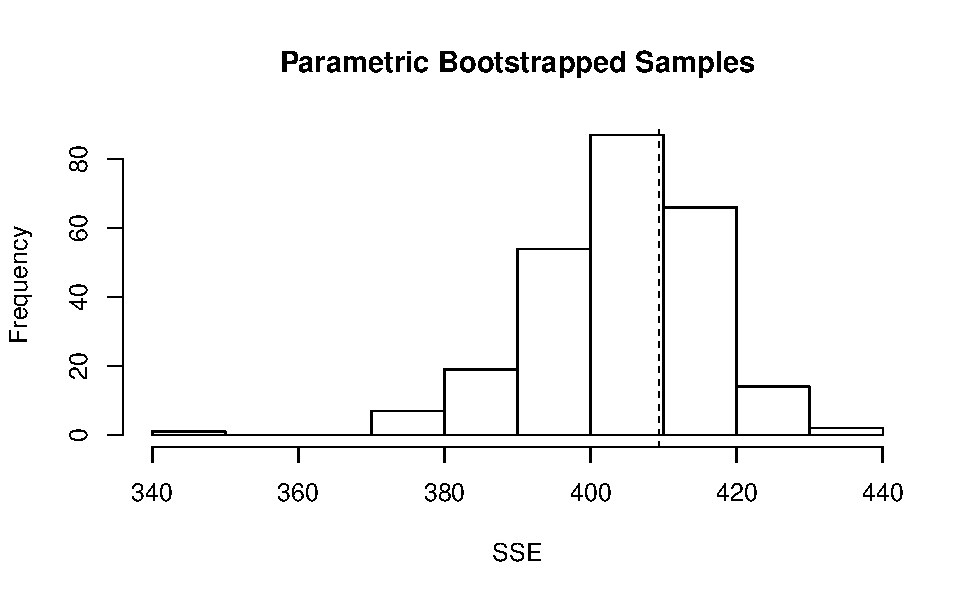
\includegraphics{Simul-Machalilla-book_files/figure-latex/fit-1.pdf}

Ahora que sabemos que nuestro mejor modelo tiene buen ajuste, podemos
usarlo para predecir la ocupación en el rango de la altitud para ver su
comportamiento en una gráfica.

\begin{Shaded}
\begin{Highlighting}[]
\NormalTok{elevrange<-}\KeywordTok{data.frame}\NormalTok{(}\DataTypeTok{elev=}\KeywordTok{seq}\NormalTok{(}\KeywordTok{min}\NormalTok{(datos2$elev),}\KeywordTok{max}\NormalTok{(datos2$elev),}\DataTypeTok{length=}\DecValTok{100}\NormalTok{)) }\CommentTok{# newdata}
\NormalTok{pred_psi <-}\KeywordTok{predict}\NormalTok{(fm7,}\DataTypeTok{type=}\StringTok{"state"}\NormalTok{,}\DataTypeTok{newdata=}\NormalTok{elevrange,}\DataTypeTok{appendData=}\OtherTok{TRUE}\NormalTok{) }
\KeywordTok{plot}\NormalTok{(Predicted~elev, pred_psi,}\DataTypeTok{type=}\StringTok{"l"}\NormalTok{,}\DataTypeTok{col=}\StringTok{"blue"}\NormalTok{,}
       \DataTypeTok{xlab=}\StringTok{"elev"}\NormalTok{,}
       \DataTypeTok{ylab=}\StringTok{"psi"}\NormalTok{)}
\KeywordTok{lines}\NormalTok{(lower~elev, pred_psi,}\DataTypeTok{type=}\StringTok{"l"}\NormalTok{,}\DataTypeTok{col=}\KeywordTok{gray}\NormalTok{(}\FloatTok{0.5}\NormalTok{))}
\KeywordTok{lines}\NormalTok{(upper~elev, pred_psi,}\DataTypeTok{type=}\StringTok{"l"}\NormalTok{,}\DataTypeTok{col=}\KeywordTok{gray}\NormalTok{(}\FloatTok{0.5}\NormalTok{))}
\end{Highlighting}
\end{Shaded}

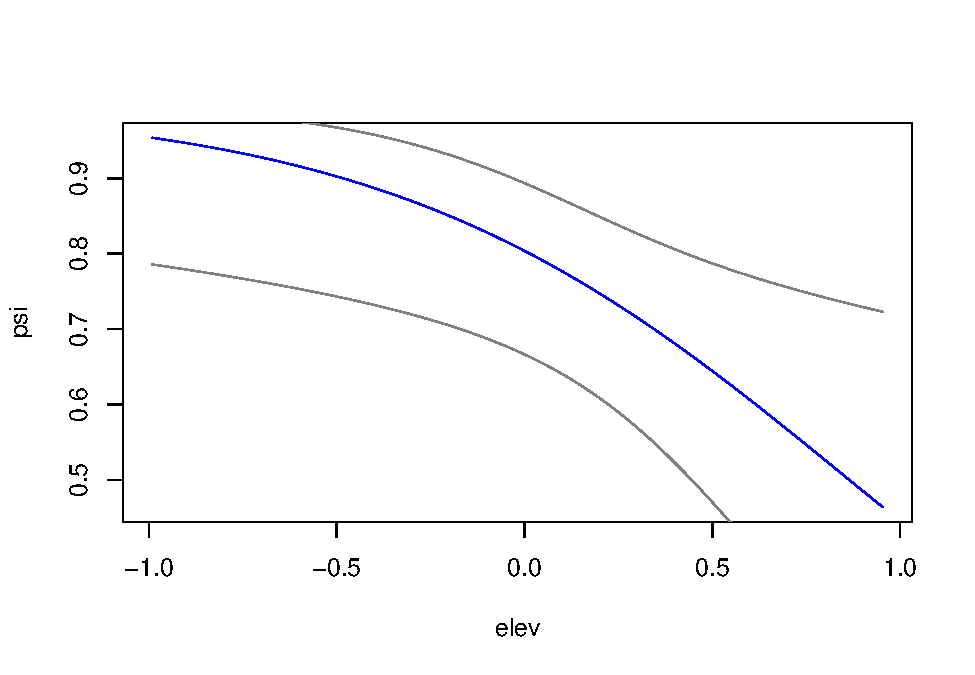
\includegraphics{Simul-Machalilla-book_files/figure-latex/graph_psi-1.pdf}

Podemos también usar el mejor modelo para predecir de forma
espacialmente explicita si tenemos los mapas. Para esto vamos a
construir mapas para cada una de nuestras covariables. Los mapas surgen
de un patrón aleatorio de puntos con distribución Poisson. Luego estos
puntos los convertimos en una superficie interpolada.

\begin{Shaded}
\begin{Highlighting}[]
\CommentTok{# lets make random maps for the three covariates}
\KeywordTok{library}\NormalTok{(raster)}
\KeywordTok{library}\NormalTok{(spatstat)}
\KeywordTok{set.seed}\NormalTok{(}\DecValTok{24}\NormalTok{) }\CommentTok{# Remove for random simulations}

\CommentTok{# CONSTRUCT ANALYSIS WINDOW USING THE FOLLOWING:}
\NormalTok{xrange=}\KeywordTok{c}\NormalTok{(-}\FloatTok{2.5}\NormalTok{, }\FloatTok{1002.5}\NormalTok{)}
\NormalTok{yrange=}\KeywordTok{c}\NormalTok{(-}\FloatTok{2.5}\NormalTok{, }\FloatTok{502.5}\NormalTok{)}
\NormalTok{window<-}\KeywordTok{owin}\NormalTok{(xrange, yrange)}

\CommentTok{# Build maps from random points and interpole in same line}
\NormalTok{elev   <-}\StringTok{ }\KeywordTok{density}\NormalTok{(}\KeywordTok{rpoispp}\NormalTok{(}\DataTypeTok{lambda=}\FloatTok{0.6}\NormalTok{, }\DataTypeTok{win=}\NormalTok{window)) }\CommentTok{# }
\NormalTok{forest <-}\StringTok{ }\KeywordTok{density}\NormalTok{(}\KeywordTok{rpoispp}\NormalTok{(}\DataTypeTok{lambda=}\FloatTok{0.2}\NormalTok{, }\DataTypeTok{win=}\NormalTok{window)) }\CommentTok{# }
\NormalTok{temp   <-}\StringTok{ }\KeywordTok{density}\NormalTok{(}\KeywordTok{rpoispp}\NormalTok{(}\DataTypeTok{lambda=}\FloatTok{0.5}\NormalTok{, }\DataTypeTok{win=}\NormalTok{window)) }\CommentTok{# }

\CommentTok{# Convert covs to raster and Put in the same stack }
\NormalTok{mapdata.m<-}\KeywordTok{stack}\NormalTok{(}\KeywordTok{raster}\NormalTok{(elev),}\KeywordTok{raster}\NormalTok{(forest), }\KeywordTok{raster}\NormalTok{(temp)) }
\KeywordTok{names}\NormalTok{(mapdata.m)<-}\StringTok{ }\KeywordTok{c}\NormalTok{(}\StringTok{"elev"}\NormalTok{, }\StringTok{"forest"}\NormalTok{, }\StringTok{"temp"}\NormalTok{) }\CommentTok{# put names to raster}

\CommentTok{# lets plot the covs maps}
\KeywordTok{plot}\NormalTok{(mapdata.m)}
\end{Highlighting}
\end{Shaded}

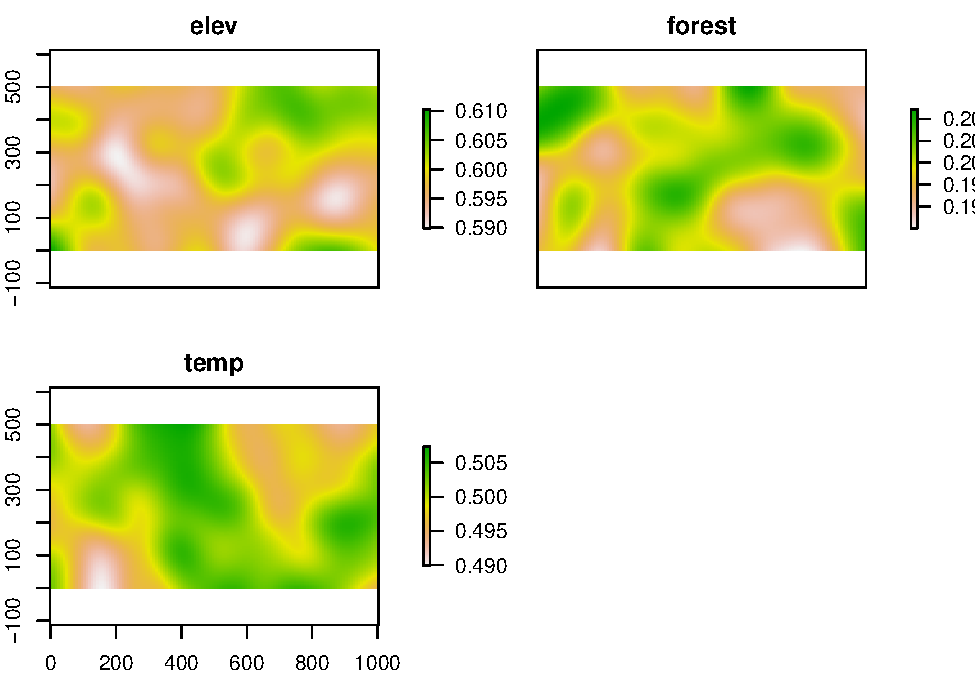
\includegraphics{Simul-Machalilla-book_files/figure-latex/spatial1-1.pdf}

Una vez tenemos nuestros mapas de covariables, los usamos para predecir
con el mejor modelo. De esta forma podemos tener un mapa con
predicciones de la ocupación y la probabilidad de detección.

\begin{Shaded}
\begin{Highlighting}[]
\CommentTok{# make the predictions }
\NormalTok{predictions_psi <-}\StringTok{ }\KeywordTok{predict}\NormalTok{(fm7, }\DataTypeTok{type=}\StringTok{"state"}\NormalTok{, }\DataTypeTok{newdata=}\NormalTok{mapdata.m) }\CommentTok{# predict psi}
\end{Highlighting}
\end{Shaded}

\begin{verbatim}
##   doing row 1000 of 16384 
##   doing row 2000 of 16384 
##   doing row 3000 of 16384 
##   doing row 4000 of 16384 
##   doing row 5000 of 16384 
##   doing row 6000 of 16384 
##   doing row 7000 of 16384 
##   doing row 8000 of 16384 
##   doing row 9000 of 16384 
##   doing row 10000 of 16384 
##   doing row 11000 of 16384 
##   doing row 12000 of 16384 
##   doing row 13000 of 16384 
##   doing row 14000 of 16384 
##   doing row 15000 of 16384 
##   doing row 16000 of 16384
\end{verbatim}

\begin{Shaded}
\begin{Highlighting}[]
\NormalTok{predictions_p   <-}\StringTok{ }\KeywordTok{predict}\NormalTok{(fm7, }\DataTypeTok{type=}\StringTok{"det"}\NormalTok{,   }\DataTypeTok{newdata=}\NormalTok{mapdata.m) }\CommentTok{# predict p}
\end{Highlighting}
\end{Shaded}

\begin{verbatim}
##   doing row 1000 of 16384 
##   doing row 2000 of 16384 
##   doing row 3000 of 16384 
##   doing row 4000 of 16384 
##   doing row 5000 of 16384 
##   doing row 6000 of 16384 
##   doing row 7000 of 16384 
##   doing row 8000 of 16384 
##   doing row 9000 of 16384 
##   doing row 10000 of 16384 
##   doing row 11000 of 16384 
##   doing row 12000 of 16384 
##   doing row 13000 of 16384 
##   doing row 14000 of 16384 
##   doing row 15000 of 16384 
##   doing row 16000 of 16384
\end{verbatim}

\begin{Shaded}
\begin{Highlighting}[]
\CommentTok{# put in the same stack}
\NormalTok{predmaps<-}\KeywordTok{stack}\NormalTok{(predictions_psi$Predicted,predictions_p$Predicted) }
\KeywordTok{names}\NormalTok{(predmaps)<-}\KeywordTok{c}\NormalTok{(}\StringTok{"psi_predicted"}\NormalTok{, }\StringTok{"p_predicted"}\NormalTok{) }\CommentTok{# put names}
\KeywordTok{plot}\NormalTok{(predmaps)}
\end{Highlighting}
\end{Shaded}

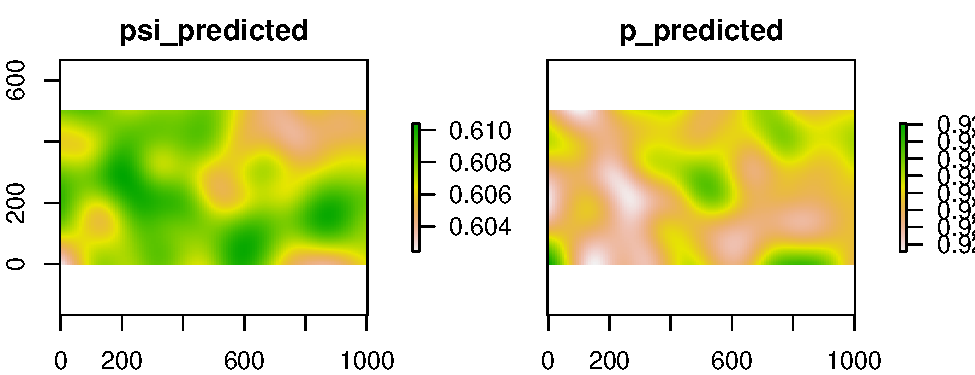
\includegraphics{Simul-Machalilla-book_files/figure-latex/spatial2-1.pdf}

\chapter{Análisis Bayesiano}\label{bayesian}

En esta parte vamos a estimar los mismos parámetros de un modelo igual
al ``mejor modelo'' el cual fue seleccionado en el procedimiento de
selección de modelos de unmarked en el capitulo anterior. Recordemos que
este modelo tiene beta1 y alpha1, alpha2, alpha3. Los parámetros que
estimaremos con el método Bayesiano los vamos a comparar con los
parámetros que ya estimamos con ML en unmarked y también los
compararemos con los parámetros reales que definimos al establecer los
datos (datos2) con la función data.fn, para ver cual de los dos métodos
de estimación (ML o Bayesiano) se acerca mas a los parámetros reales.

\section{Generando los datos}\label{generando-los-datos-1}

De nuevo usaremos un diseño tipo TEAM (\url{http://www.teamnetwork.org})
con 60 sitios de muestreo y 30 visitas repetidas, que equivalen a los 30
días en que las camaras permenecen activas en campo. Nuestra especie
sigue siendo la misma, el venado de cola blanca. Para este ejemplo
asumiremos que la detección es 0.6, la ocupacion 0.8 y las interacciones
son sencillas con la altitud como la unica covariable que explica la
ocupación. Pero para la deteccion hay una relación mas compleja,
asumiendo que hay una leve interacción entre las covariables de la
observación. Para la observación la altitud y temperatura interactuan
entre si. Tambien observe como la altitud influye en direcciones
opuestas con un signo positivo en la altitud para la detección y
negativo para la ocupación.

\begin{Shaded}
\begin{Highlighting}[]
\CommentTok{# ### Generate a new data set or use the same}
\CommentTok{# # ****************************************}
\CommentTok{# set.seed(148)}
\CommentTok{# data <- data.fn(show.plot = T)    # Default arguments}
\CommentTok{# str(data)                         # Look at the object}
\CommentTok{# we are oing to use the data from datos2 object}

\NormalTok{### Fit same model with JAGS, using library jagsUI}
\CommentTok{# ************************************************}
\CommentTok{# Bundle data}
\NormalTok{win.data <-}\StringTok{ }\KeywordTok{list}\NormalTok{(}\DataTypeTok{y =} \NormalTok{datos2$y, }
                 \DataTypeTok{M =} \KeywordTok{nrow}\NormalTok{(datos2$y), }
                 \DataTypeTok{J =} \KeywordTok{ncol}\NormalTok{(datos2$y), }
                 \DataTypeTok{elev =} \NormalTok{datos2$elev, }
                 \DataTypeTok{forest =} \NormalTok{datos2$forest, }
                 \DataTypeTok{temp =} \NormalTok{datos2$temp)}
\CommentTok{# str(win.data)}


\CommentTok{# # Specify model in BUGS language}
\CommentTok{# sink("model22.txt")}
\CommentTok{# cat("}
\CommentTok{# model \{}
\CommentTok{# }
\CommentTok{# # Priors}
\CommentTok{# mean.p ~ dunif(0, 1)        # Detection intercept on prob. scale}
\CommentTok{# alpha0 <- logit(mean.p)     # same on logit scale}
\CommentTok{# mean.psi ~ dunif(0, 1)      # Occupancy intercept on prob. scale}
\CommentTok{# beta0 <- logit(mean.psi)    # same on logit scale}
\CommentTok{# for(k in 1:3)\{              # 2 detection covariates + 1 interact}
\CommentTok{#     alpha[k] ~ dnorm(0, 0.01) # Covariates on logit(detection)}
\CommentTok{# #   alpha[k] ~ dnorm(0, 0.05) # Covariates on logit(detection)}
\CommentTok{# #   alpha[k] ~ dunif(-10, 10) # Covariates on logit(detection)}
\CommentTok{# \}}
\CommentTok{# }
\CommentTok{# for(k in 1:1)\{                # 2 occupancy covariates + 1 interact}
\CommentTok{#     beta[k] ~ dnorm(0, 0.01)  # Covariates on logit(occupancy)}
\CommentTok{# #   beta[k] ~ dnorm(0, 0.05)  # Covariates on logit(occupancy)}
\CommentTok{# #   beta[k] ~ dunif(-10, 10)  # Covariates on logit(occupancy)}
\CommentTok{# \}}
\CommentTok{# }
\CommentTok{# # Translation of the occupancy parameters in unmarked into those for BUGS:}
\CommentTok{# # (Intercept)         (beta0 in BUGS)}
\CommentTok{# # elev                (beta[1])}
\CommentTok{# # forest              (beta[2])}
\CommentTok{# # temp                (beta[3])}
\CommentTok{# # elev:forest         (beta[4])}
\CommentTok{# # elev:temp           (beta[5])}
\CommentTok{# # forest:temp         (beta[6])}
\CommentTok{# # elev:forest:temp    (beta[7])}
\CommentTok{# }
\CommentTok{# }
\CommentTok{# # Likelihood}
\CommentTok{# for (i in 1:M) \{}
\CommentTok{#   # True state model for the partially observed true state}
\CommentTok{#   z[i] ~ dbern(psi[i])                      # True occupancy z at site i}
\CommentTok{#   logit(psi[i]) <- beta0 +                  # occupancy (psi) intercept}
\CommentTok{#     beta[1] * elev[i] #+                     # elev}
\CommentTok{#     #beta[2] * forest[i] #+                  # forest}
\CommentTok{#     #beta[3] * elev[i] * forest[i]          # elev:forest}
\CommentTok{#     #beta[4] * elev[i] * temp[i] +          # elev:temp}
\CommentTok{#     #beta[5] * temp[i] +                    # temp}
\CommentTok{#     #beta[6] * forest[i] * temp[i] +        # forest:temp}
\CommentTok{#     #beta[7] * elev[i] * forest[i] * temp[i]   # elev:forest:temp}
\CommentTok{# }
\CommentTok{#    for (j in 1:J) \{}
\CommentTok{#       # Observation model for the actual observations}
\CommentTok{#       y[i,j] ~ dbern(p.eff[i,j])      # Detection-nondetection at i and j}
\CommentTok{#       p.eff[i,j] <- z[i] * p[i,j]}
\CommentTok{#       logit(p[i,j]) <- alpha0 +             # detection (p) intercept}
\CommentTok{#          alpha[1] * elev[i] +               # effect of elevation on p}
\CommentTok{#          alpha[2] * temp[i,j] +             # effect of temp on p}
\CommentTok{#          alpha[3] * elev[i] * temp[i,j]     # effect of elev:temp on p}
\CommentTok{#    \}}
\CommentTok{# \}}
\CommentTok{# }
\CommentTok{# # Derived quantities}
\CommentTok{# sumZ <- sum(z[])      # Number of occupied sites among those studied}
\CommentTok{# occ.fs <- sum(z[])/M  # proportion of occupied sites among those studied}
\CommentTok{# logit.psi <- beta0    # For comparison with unmarked}
\CommentTok{# logit.p <- alpha0     # For comparison with unmarked}
\CommentTok{# \}}
\CommentTok{# ",fill = TRUE)}
\CommentTok{# sink()}


\KeywordTok{library}\NormalTok{(jagsUI)}
\CommentTok{# library(R2jags)}
\CommentTok{# Initial values}
\NormalTok{zst <-}\StringTok{ }\KeywordTok{apply}\NormalTok{(datos2$y, }\DecValTok{1}\NormalTok{, max)}
\NormalTok{inits <-}\StringTok{ }\NormalTok{function()\{}\KeywordTok{list}\NormalTok{(}\DataTypeTok{z =} \NormalTok{zst, }
                         \DataTypeTok{mean.psi =} \KeywordTok{runif}\NormalTok{(}\DecValTok{1}\NormalTok{), }
                         \DataTypeTok{mean.p =} \KeywordTok{runif}\NormalTok{(}\DecValTok{1}\NormalTok{), }
                         \DataTypeTok{alpha =} \KeywordTok{rnorm}\NormalTok{(}\DecValTok{3}\NormalTok{), }\CommentTok{# adjust here}
                         \DataTypeTok{beta =} \KeywordTok{rnorm}\NormalTok{(}\DecValTok{1}\NormalTok{))\} }\CommentTok{# adjust here}

\CommentTok{# Parameters monitored}
\NormalTok{params <-}\StringTok{ }\KeywordTok{c}\NormalTok{(}\StringTok{"sumZ"}\NormalTok{, }\StringTok{"occ.fs"}\NormalTok{, }\StringTok{"logit.psi"}\NormalTok{, }\StringTok{"logit.p"}\NormalTok{, }\StringTok{"alpha"}\NormalTok{, }\StringTok{"beta"}\NormalTok{)}

\CommentTok{# MCMC settings}
\CommentTok{# ni <- 50000   ;   nt <- 10   ;   nb <- 1000   ;   nc <- 3}
 \NormalTok{ni <-}\StringTok{ }\DecValTok{600}   \NormalTok{;   nt <-}\StringTok{ }\DecValTok{1}   \NormalTok{;   nb <-}\StringTok{ }\DecValTok{100}   \NormalTok{;   nc <-}\StringTok{ }\DecValTok{3}

\CommentTok{# Call JAGS from R (ART 260 sec with norm(), 480 with unif(-10,10)) }
\CommentTok{# and summarize posteriors}
\KeywordTok{system.time}\NormalTok{(out22 <-}\StringTok{ }\KeywordTok{jags}\NormalTok{(win.data, inits, }\DataTypeTok{parameters.to.save =} \NormalTok{params,}
                      \DataTypeTok{model.file =} \StringTok{"C:/Users/Diego/Documents/CodigoR/IntroOccupancy/model22.txt"}\NormalTok{, }
                          \DataTypeTok{n.chains =} \NormalTok{nc, }
                          \DataTypeTok{n.thin =} \NormalTok{nt, }
                          \DataTypeTok{n.iter =} \NormalTok{ni, }
                          \DataTypeTok{n.burnin =} \NormalTok{nb, }
                          \DataTypeTok{parallel =} \NormalTok{T))}
\end{Highlighting}
\end{Shaded}

\begin{verbatim}
## 
## Processing function input....... 
## 
## Done. 
##  
## Beginning parallel processing using 2 cores. Console output will be suppressed.
## 
## Parallel processing completed.
## 
## Calculating statistics....... 
## 
## Done.
\end{verbatim}

\begin{verbatim}
##    user  system elapsed 
##    0.08    0.02   33.48
\end{verbatim}

\begin{Shaded}
\begin{Highlighting}[]
\CommentTok{# See model diagnistics and convergence }
\KeywordTok{library}\NormalTok{(mcmcplots)}
\KeywordTok{library}\NormalTok{(ggmcmc)}
\NormalTok{fit22.mcmc <-}\StringTok{ }\KeywordTok{as.mcmc.list}\NormalTok{(out22$samples)}
\NormalTok{bayes.mod.fit.gg <-}\StringTok{ }\KeywordTok{ggs}\NormalTok{(fit22.mcmc) }\CommentTok{#convert to ggmcmc}
\KeywordTok{ggs_running}\NormalTok{(bayes.mod.fit.gg)}\CommentTok{# check if chains approach target distrib. }
\end{Highlighting}
\end{Shaded}

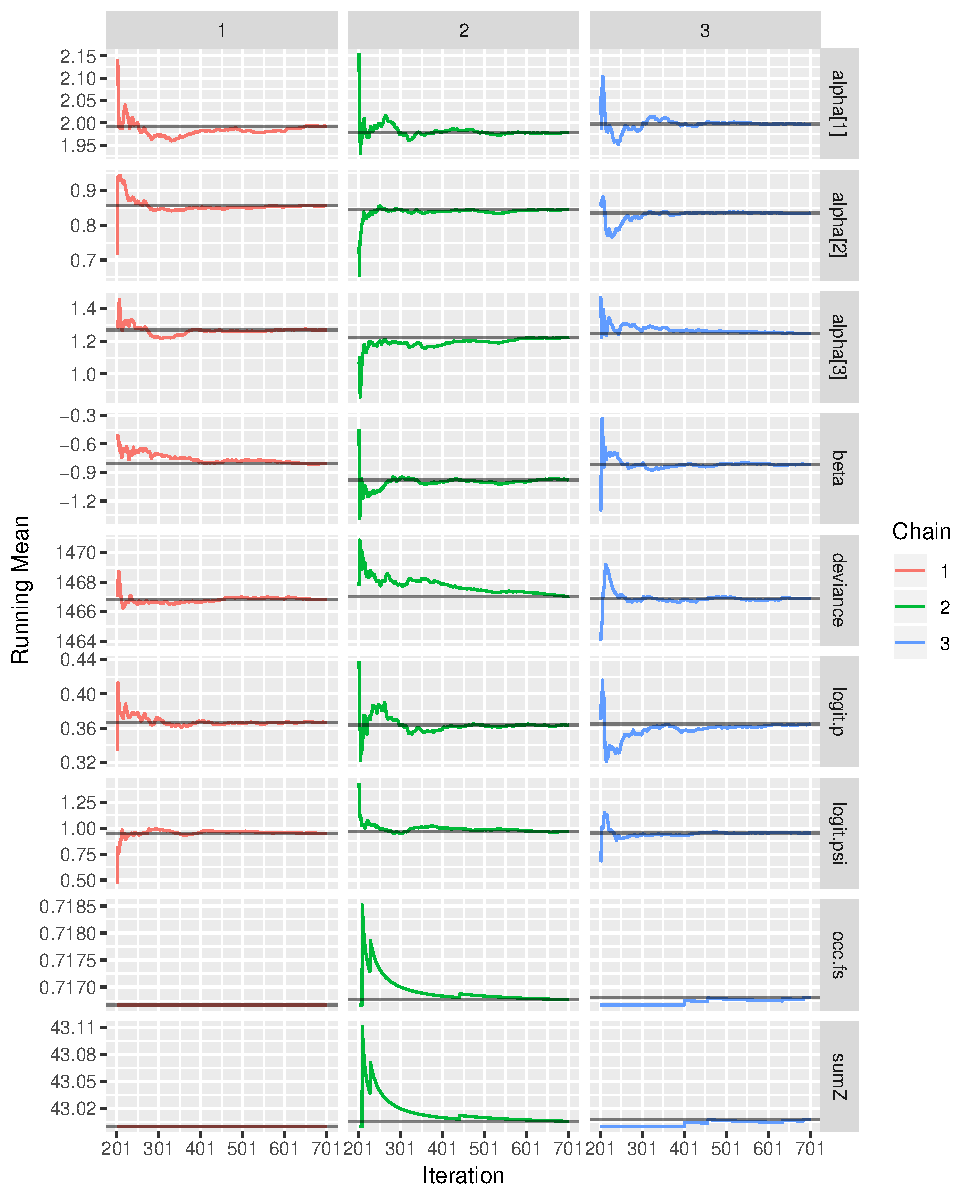
\includegraphics{Simul-Machalilla-book_files/figure-latex/Bayesian-1.pdf}

\begin{Shaded}
\begin{Highlighting}[]
\CommentTok{# denplot(fit22.mcmc, parms = c("beta", }
\CommentTok{#                               "alpha[1]", "alpha[2]", "alpha[3]", }
\CommentTok{#                               "logit.psi", "logit.p" ))}
\CommentTok{# traplot(fit22.mcmc)}
\CommentTok{# ggs_density(bayes.mod.fit.gg)}

\KeywordTok{xyplot}\NormalTok{(out22)        }\CommentTok{# assess within-chain convergence}
\end{Highlighting}
\end{Shaded}

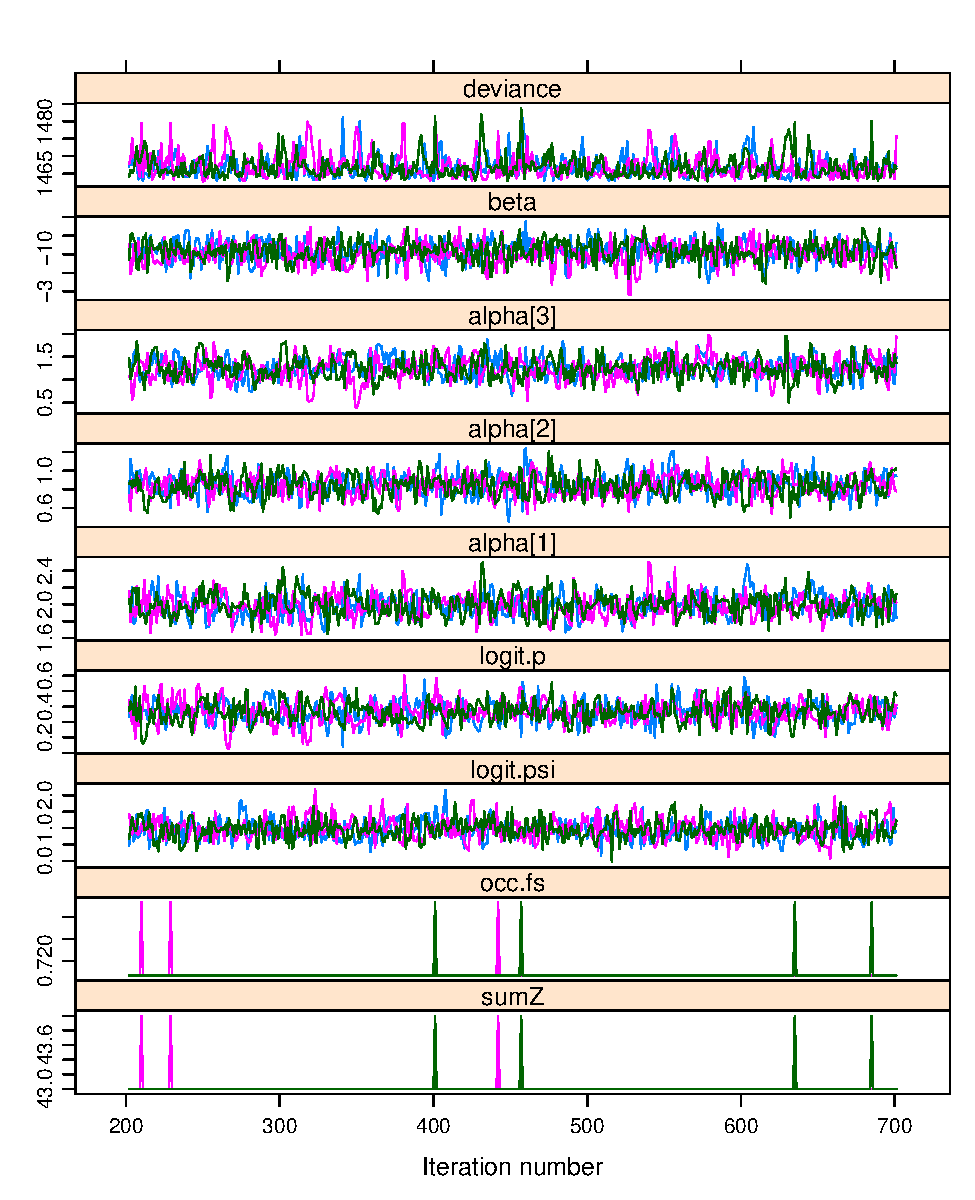
\includegraphics{Simul-Machalilla-book_files/figure-latex/Bayesian-2.pdf}

\begin{Shaded}
\begin{Highlighting}[]
\KeywordTok{densityplot}\NormalTok{(out22)  }\CommentTok{# shape of the posterior distribution}
\end{Highlighting}
\end{Shaded}

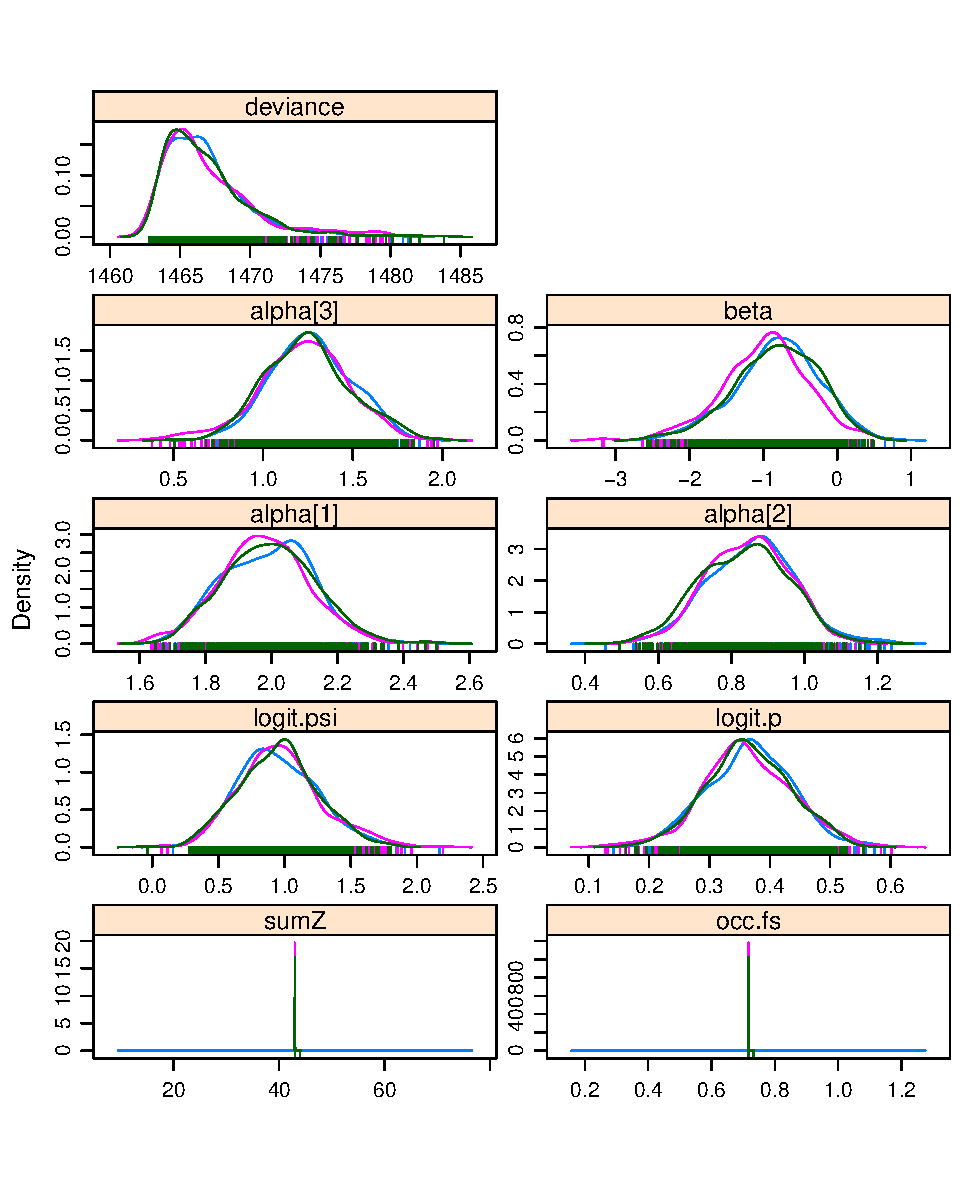
\includegraphics{Simul-Machalilla-book_files/figure-latex/Bayesian-3.pdf}

\begin{Shaded}
\begin{Highlighting}[]
\CommentTok{# see model result and estimates  }
\KeywordTok{print}\NormalTok{(out22, }\DecValTok{3}\NormalTok{)}
\end{Highlighting}
\end{Shaded}

\begin{verbatim}
## JAGS output for model 'C:/Users/Diego/Documents/CodigoR/IntroOccupancy/model22.txt', generated by jagsUI.
## Estimates based on 3 chains of 600 iterations,
## burn-in = 100 iterations and thin rate = 1,
## yielding 1500 total samples from the joint posterior. 
## MCMC ran in parallel for 0.557 minutes at time 2016-07-24 10:44:15.
## 
##               mean    sd     2.5%      50%    97.5% overlap0     f  Rhat
## sumZ        46.032 0.176   46.000   46.000   47.000    FALSE 1.000 1.001
## occ.fs       0.767 0.003    0.767    0.767    0.783    FALSE 1.000 1.001
## logit.psi    1.178 0.324    0.596    1.153    1.842    FALSE 1.000 1.000
## logit.p      0.407 0.071    0.270    0.407    0.543    FALSE 1.000 1.001
## alpha[1]     2.139 0.152    1.853    2.134    2.446    FALSE 1.000 1.002
## alpha[2]     0.898 0.125    0.668    0.894    1.144    FALSE 1.000 1.002
## alpha[3]     1.680 0.248    1.205    1.677    2.167    FALSE 1.000 1.003
## beta        -1.449 0.660   -2.803   -1.426   -0.190    FALSE 0.989 1.006
## deviance  1589.455 3.627 1585.468 1588.515 1600.360    FALSE 1.000 1.003
##           n.eff
## sumZ       1500
## occ.fs     1500
## logit.psi  1500
## logit.p     988
## alpha[1]   1500
## alpha[2]    987
## alpha[3]    859
## beta        352
## deviance   1061
## 
## Successful convergence based on Rhat values (all < 1.1). 
## Rhat is the potential scale reduction factor (at convergence, Rhat=1). 
## For each parameter, n.eff is a crude measure of effective sample size. 
## 
## overlap0 checks if 0 falls in the parameter's 95% credible interval.
## f is the proportion of the posterior with the same sign as the mean;
## i.e., our confidence that the parameter is positive or negative.
## 
## DIC info: (pD = var(deviance)/2) 
## pD = 6.6 and DIC = 1596.027 
## DIC is an estimate of expected predictive error (lower is better).
\end{verbatim}

\begin{Shaded}
\begin{Highlighting}[]
\CommentTok{# store in tmp coefficients from best ML model}
\NormalTok{tmp <-}\StringTok{ }\KeywordTok{summary}\NormalTok{(fm7)}
\end{Highlighting}
\end{Shaded}

\begin{verbatim}
## 
## Call:
## occu(formula = ~elev + temp + elev:temp ~ elev, data = umf)
## 
## Occupancy (logit-scale):
##             Estimate    SE     z  P(>|z|)
## (Intercept)     1.18 0.326  3.62 0.000291
## elev           -1.41 0.624 -2.26 0.023548
## 
## Detection (logit-scale):
##             Estimate     SE     z  P(>|z|)
## (Intercept)    0.407 0.0735  5.54 3.03e-08
## elev           2.140 0.1494 14.32 1.66e-46
## temp           0.900 0.1262  7.14 9.68e-13
## elev:temp      1.680 0.2514  6.68 2.34e-11
## 
## AIC: 1656.533 
## Number of sites: 60
## optim convergence code: 0
## optim iterations: 37 
## Bootstrap iterations: 0
\end{verbatim}

\begin{Shaded}
\begin{Highlighting}[]
\NormalTok{modestimates <-}\StringTok{ }\KeywordTok{cbind}\NormalTok{(}\KeywordTok{rbind}\NormalTok{(tmp$state[}\DecValTok{1}\NormalTok{:}\DecValTok{2}\NormalTok{], tmp$det[}\DecValTok{1}\NormalTok{:}\DecValTok{2}\NormalTok{]), }
                \DataTypeTok{Post.mean =} \NormalTok{out22$summary[}\KeywordTok{c}\NormalTok{(}\DecValTok{3}\NormalTok{, }\DecValTok{8}\NormalTok{, }\DecValTok{4}\NormalTok{:}\DecValTok{7}\NormalTok{), }\DecValTok{1}\NormalTok{],}
                \DataTypeTok{Post.sd   =} \NormalTok{out22$summary[}\KeywordTok{c}\NormalTok{(}\DecValTok{3}\NormalTok{, }\DecValTok{8}\NormalTok{, }\DecValTok{4}\NormalTok{:}\DecValTok{7}\NormalTok{), }\DecValTok{2}\NormalTok{] )}

\CommentTok{# fix the(logit-scale) in unmarked }
\NormalTok{modestimates[}\DecValTok{1}\NormalTok{,}\DecValTok{1}\NormalTok{]<-}\StringTok{ }\KeywordTok{plogis}\NormalTok{(modestimates[}\DecValTok{1}\NormalTok{,}\DecValTok{1}\NormalTok{])}
\NormalTok{modestimates[}\DecValTok{3}\NormalTok{,}\DecValTok{1}\NormalTok{]<-}\StringTok{ }\KeywordTok{plogis}\NormalTok{(modestimates[}\DecValTok{3}\NormalTok{,}\DecValTok{1}\NormalTok{])}

\CommentTok{# fix the(logit-scale) in Bayes in logit.psi  logit.p}
\NormalTok{modestimates[}\DecValTok{1}\NormalTok{,}\DecValTok{3}\NormalTok{]<-}\StringTok{ }\KeywordTok{plogis}\NormalTok{(modestimates[}\DecValTok{1}\NormalTok{,}\DecValTok{3}\NormalTok{])}
\NormalTok{modestimates[}\DecValTok{3}\NormalTok{,}\DecValTok{3}\NormalTok{]<-}\StringTok{ }\KeywordTok{plogis}\NormalTok{(modestimates[}\DecValTok{3}\NormalTok{,}\DecValTok{3}\NormalTok{])}

\CommentTok{# get real values from datos2 object}
\NormalTok{real<-}\StringTok{ }\KeywordTok{rbind}\NormalTok{(datos2$mean.occupancy, datos2$beta1, datos2$mean.detection,}
             \NormalTok{datos2$alpha1, datos2$alpha2, datos2$alpha3)}
\end{Highlighting}
\end{Shaded}

\section{Comparando los valores reales y los estimados de ML y
Bayesiano}\label{comparando-los-valores-reales-y-los-estimados-de-ml-y-bayesiano}

Veamos que tan cerca están los estimados de los valores reales,
comparando el valor real con el estimado de Máxima Verosimilitud
(columnas 2 y 3) y el estimado Bayesiano (columnas 4 y 5).

\begin{Shaded}
\begin{Highlighting}[]
\NormalTok{### see if the values are close to real values}
\NormalTok{compare <-}\StringTok{ }\KeywordTok{cbind}\NormalTok{(real, modestimates) }\CommentTok{# put both in same table}
\CommentTok{# put names to rows}
\KeywordTok{rownames}\NormalTok{(compare) <-}\StringTok{ }\KeywordTok{c}\NormalTok{(}\StringTok{"psi"}\NormalTok{,}\StringTok{"beta"}\NormalTok{,}\StringTok{"p"}\NormalTok{,}\StringTok{"alpha1"}\NormalTok{,}\StringTok{"alpha2"}\NormalTok{, }\StringTok{"alpha3"}\NormalTok{)}

\CommentTok{# print comparing table}
\KeywordTok{library}\NormalTok{(knitr)}
\KeywordTok{kable}\NormalTok{(compare)}
\end{Highlighting}
\end{Shaded}

\begin{tabular}{l|r|r|r|r|r}
\hline
  & real & Estimate & SE & Post.mean & Post.sd\\
\hline
psi & 0.8 & 0.7653197 & 0.3262574 & 0.7645364 & 0.3243590\\
\hline
beta & -1.5 & -1.4129006 & 0.6239572 & -1.4491027 & 0.6596557\\
\hline
p & 0.6 & 0.6004304 & 0.0735178 & 0.6003412 & 0.0712036\\
\hline
alpha1 & 2.0 & 2.1395071 & 0.1494144 & 2.1390329 & 0.1517535\\
\hline
alpha2 & 1.0 & 0.9003900 & 0.1261927 & 0.8977662 & 0.1249009\\
\hline
alpha3 & 1.5 & 1.6801587 & 0.2513946 & 1.6796383 & 0.2483400\\
\hline
\end{tabular}

\chapter{Información de la sessión de R y los paquetes
usados}\label{informacion-de-la-session-de-r-y-los-paquetes-usados}

\begin{Shaded}
\begin{Highlighting}[]
\KeywordTok{sessionInfo}\NormalTok{()}
\end{Highlighting}
\end{Shaded}

\begin{verbatim}
## R version 3.3.0 (2016-05-03)
## Platform: x86_64-w64-mingw32/x64 (64-bit)
## Running under: Windows 7 x64 (build 7601) Service Pack 1
## 
## locale:
## [1] LC_COLLATE=English_United States.1252 
## [2] LC_CTYPE=English_United States.1252   
## [3] LC_MONETARY=English_United States.1252
## [4] LC_NUMERIC=C                          
## [5] LC_TIME=English_United States.1252    
## 
## attached base packages:
## [1] stats     graphics  grDevices utils     datasets  methods   base     
## 
## other attached packages:
##  [1] ggmcmc_1.1      ggplot2_2.1.0   tidyr_0.5.1     dplyr_0.5.0    
##  [5] mcmcplots_0.4.2 coda_0.18-1     jagsUI_1.4.2    spatstat_1.46-1
##  [9] rpart_4.1-10    nlme_3.1-128    raster_2.5-8    sp_1.2-3       
## [13] unmarked_0.11-0 Rcpp_0.12.6     lattice_0.20-33 reshape_0.8.5  
## [17] knitr_1.13     
## 
## loaded via a namespace (and not attached):
##  [1] denstrip_1.5.3     reshape2_1.4.1     colorspace_1.2-6  
##  [4] miniUI_0.1.1       htmltools_0.3.5    yaml_2.1.13       
##  [7] mgcv_1.8-13        DBI_0.4-1          plyr_1.8.4        
## [10] stringr_1.0.0      munsell_0.4.3      gtable_0.2.0      
## [13] codetools_0.2-14   evaluate_0.9       labeling_0.3      
## [16] GGally_1.2.0       httpuv_1.3.3       parallel_3.3.0    
## [19] highr_0.6          xtable_1.8-2       tensor_1.5        
## [22] scales_0.4.0       formatR_1.4        abind_1.4-5       
## [25] mime_0.5           deldir_0.1-12      rjags_4-6         
## [28] digest_0.6.9       stringi_1.1.1      bookdown_0.1      
## [31] shiny_0.13.2       polyclip_1.5-6     grid_3.3.0        
## [34] tools_3.3.0        magrittr_1.5       goftest_1.0-3     
## [37] lazyeval_0.2.0     tibble_1.1         Matrix_1.2-6      
## [40] assertthat_0.1     rmarkdown_1.0.9001 rstudioapi_0.6    
## [43] R6_2.1.2           sfsmisc_1.1-0
\end{verbatim}

\bibliography{packages,book,refs}


\end{document}
